
\documentclass[a4paper, 11pt]{report}
\usepackage{graphicx}
\usepackage{mystyle}

\usepackage{hyperref}

\newcommand\blankpage{%
    \null
    \thispagestyle{empty}%
    \addtocounter{page}{-1}%
    \newpage}

\fancypagestyle{plain}{
\fancyhead[L]{Valorisation de l'open source}
\fancyhead[R]{Cesi Alternance}
\fancyfoot[L]{Matthieu Balondrade}
\fancyfoot[R]{MSI 2019}}
\pagestyle{plain}
\makenoidxglossaries


\definecolor{witchhaze}{RGB}{255, 246, 143}
\definecolor{burntorange}{RGB}{211, 84, 0}
\newglossaryentry{latex}
{
        name=Latex,
        description={Is a mark up language specially suited for 
scientific documents}
}
\newglossaryentry{open source}
{
		name=Open Source,
		description={La désignation open source, ou « code source ouvert », s'applique aux logiciels (et s'étend maintenant aux œuvres de l'esprit) dont la licence respecte des critères précisément établis par l'\acrfull{osi}, c'est-à-dire les possibilités de libre redistribution, d'accès au code source et de création de travaux dérivés
	}
}

\newglossaryentry{Creative Commons}
{
	name=Creative Commons,
	description={
		https://creativecommons.org/licenses/by-nd/2.0
	}
}

\newglossaryentry{framework}
{
	name=Framework,
	description={
		Un framework est un ensemble d'outils et de composants logiciels organisés conformément à un plan d'architecture et des patterns, l'ensemble formant ou promouvant un "squelette" de programme, un canevas. Il est souvent fourni sous la forme d'une bibliothèque logicielle et accompagné du plan de l'architecture cible du framework.
		Un framework est conçu en vue d'aider les programmeurs dans leur travail. L'organisation du framework vise la productivité maximale du programmeur qui va l'utiliser.
	}
}

\newglossaryentry{apache}
{
	name=Apache,
	description={
		L'Apache Software Foundation (ASF) est une organisation à but non lucratif qui développe des logiciels open source sous la licence Apache, dont le renommé serveur web Apache HTTP Server. Elle a été créée en juin 1999 dans le Delaware aux États-Unis.
	}
}
\newacronym{osi}{OSI}{Open Source Initiative}
\newacronym{floss}{FLOSS}{Free/Libre and Open Source Software}
\newacronym{fsf}{FSF}{Free Software Foundation}
\newacronym{bsd}{BSD}{Berkeley Software Distribution}
\newacronym{gnu gpl}{GNU GPL}{GNU General Public Licence}
\newacronym{saas}{SaaS}{Software as a Service}



\title{\Huge \color{burntorange}{Valorisation de l'open source en tant qu'éditeur}}
\author{\Large Matthieu \bsc{Balondrade} }
\date{\Large 5 Février 2020}

\begin{document}
\maketitle
\afterpage{\blankpage}
\tableofcontents
\listoffigures
\printnoidxglossaries
\printglossary[type=\acronymtype]

\chapter*{\color{burntorange}{Preface}}
	\section*{Remerciement}
	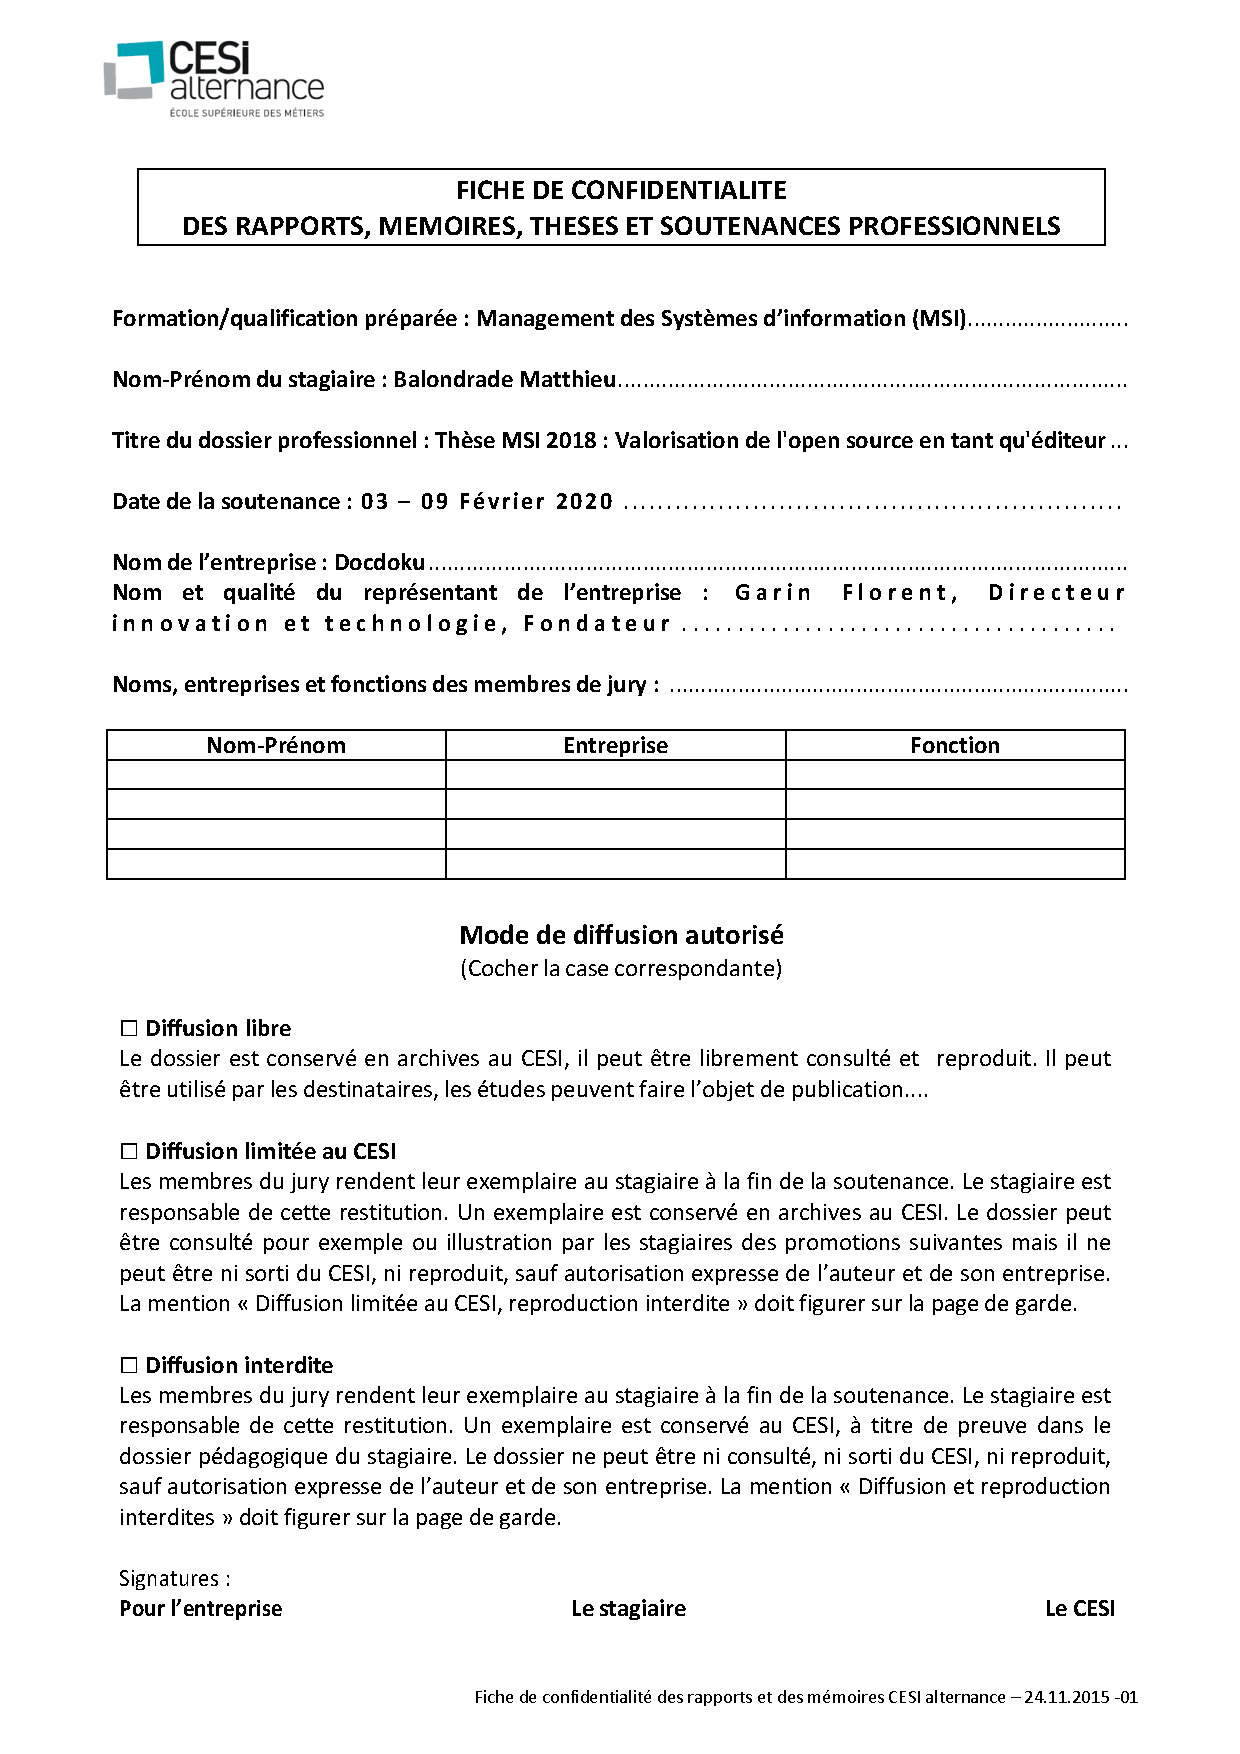
\includepdf[pages=-]{confidentialite.pdf} % Fiche de confidentialité
\chapter*{Abstract}

\section*{English}
	
	\paragraph*{Introduction\\}

	This document aims to expose the different arguments on how to enhance the open source work as an editor and promote open source to be the main solution picked by potential consummers.

	Open source is very important in IT and moreover is a school of thought. Understanding how and why it matters will increase the number of contributions and help the IT's world. That is why I offer you a first step into open source from the editor's side.

	My hypotheses are that we can improve the promotion made to the open source from the hosting platform. We can optimize the human ressources that contribute to the project by attributing their work and specilizing them and also that we need to raise awareness of the world about the open source importance.

	\paragraph*{First part\\}

	I did my research, over all, about the open source and specificaly the aspect that can be improved in order to make it the best solution for its consummers.
	My studies gather informations about the open source's consummer: it expectations, it needs and requirements. You'll also find more about the editor and the business model that works with the open source project.

	In order to improve the open source community sharing work, I did research about the collective intelligence from books and the horizontal management of project.

	Lastly, I found some aspect on what kind of marketing could be done to promote the open source solutions.

	Once this research done, I started to ask people's opinion about my thought related to open source.

	\paragraph*{Second part\\}

	I did some interview with people concerned by open source. In addition a form was sent and treated by 40 persons.

	The answers reflect multiple improvements that can be done on the communication aspect in general, whether it is for the consummer's expectation that needs to be heard or the editor that should guide contributions.

	It has also enlightened my vision about the collective aspect and project management of the open source work. I understood that all contributions made to the open source are on a voluntary basis, hence the discrepency between my expectations to attribute specific work to contributors on the project and their free will.

	Make companies and developers aware of the importance of open source and its interests is a fact that emerged from this study.

	Finally, despite the marketing aspect coming from the "open" part of the open source, a classic marketing to promote the product is still required.

	I was now able to compare my opinion to people's one in order to answer my hypotheses and give an anwser for editors to enhance the open source.

	\paragraph*{Hypotheses answered\\}

	This confrontation revealed that my hypothesis about the awareness of people that need to be raised is correct but does concern more the companies and the developers rather than the entire world.

	I was wrong about the optimization of the human ressources by attributing their work using collective intelligence and managing them because contributors can not be managed.

	Hosting platforms can be improved, not in the way that I expected, but on the documentation aspect that will help people to contribute easily. So my hypothesis about that is partially valid

	\paragraph*{Conclusion\\}

	To begin your journey in open source as an editor, this study will show you some levers that should be considered such as communications, awareness of people and companies and guides for first contributors.

\section*{Français}

	\paragraph*{Introduction\\}

	Ce document a pour but d'exposer les différents arguments sur la façon d'améliorer l'open source en tant qu'éditeur et de promouvoir celui-ci afin d'en faire la solution principale pour les consommateurs.

	Je vous parle de l'open source car il s'agit d'un sujet très important pour l'informatique mais également d'un mouvement de pensée.
	En comprenant le pourquoi et le comment de son importance, cela augmentera peut-être le nombre total de contributions et améliorera le monde de l'informatique. C'est pourquoi je vous parle de l'open source.

	Mon hypothèse est que nous pouvons améliorer la promotion faite à l'open source à partir de la plateforme d'hébergement. Nous pouvons optimiser les ressources humaines qui contribuent au projet en attribuant leur travail et en les spécialisant. Egalement, je pense que nous avons besoin de sensibiliser le monde à l'importance de l'open source.

	\paragraph*{Première partie\\}

	J'ai fais mes recherches sur l'open source et plus particulièrement sur ce qui peut être amélioré pour en faire la meilleure solution aux yeux des consommateurs.

	Mes études rassemblent des informations sur le consommateur de l'open source : ses attentes, ses besoins et ses exigences. Vous y trouverez des informations sur l'éditeur et le modèle économique qui fonctionne avec le projet open source.

	Afin d'améliorer le travail de partage de la communauté open source, j'ai fait des recherches sur l'intelligence collective issue d'ouvrages et la gestion horizontale de projet.

	Enfin, j'ai trouvé un aspect sur le type de marketing qui pourrait être fait pour promouvoir les solutions open sources.

	Une fois cette recherche effectuée, j'ai commencé à demander aux gens leur opinion sur le sujet.

	\paragraph*{Deuxième partie\\}

	J'ai fait quelques interviews avec des personnes concernées par l'open source. De plus, un formulaire a été envoyé et traité par 40 personnes.

	Les réponses reflètent les multiples améliorations qui peuvent être apportées sur l'aspect communication en général, que ce soit pour les attentes du consommateur qui doivent être entendues ou de l'éditeur qui doit guider les contributions.

	Cela a également éclairé ma vision sur l'aspect collectif et la gestion de projet du travail open source. J'ai compris que toutes les contributions faites à l'open source le sont sur une base volontaire, d'où le décalage entre mes attentes d'attribuer un travail spécifique aux contributeurs sur le projet et leur libre-arbitre.

	Faire prendre conscience aux entreprises et aux développeurs de l'importance de l'open source et de ses intérêts est un fait qui ressort de cette étude.

	Enfin, malgré l'aspect marketing venant de la partie "open" de l'open source, un marketing classique pour promouvoir le produit open source est encore nécessaire.

	J'ai donc pu comparer mon opinion à celle des gens afin de répondre à mes hypothèses et de donner une réponse aux éditeurs pour améliorer l'open source.

	\paragraph*{Réponses aux hypothèses\\}

	Cette confrontation a révélé que mon hypothèse sur la prise de conscience des personnes à sensibiliser est correcte, mais qu'elle concerne plus les entreprises et les développeurs que le monde entier.

	Je me suis trompé sur l'optimisation des ressources humaines en pensant attribuer leur travail par l'intelligence collective, car les contributeurs ne peuvent pas être managés.

	Les plateformes d'hébergement peuvent être améliorées, pas de la manière que j'attendais, mais plus sur l'aspect documentation qui aidera les gens à contribuer facilement. Mon hypothèse à ce sujet est donc partiellement valable.

	\paragraph*{Conclusion\\}

	Pour débuter votre parcours dans l'open source en tant qu'éditeur, cette étude vous montrera quelques leviers à considérer tels que la communication, la sensibilisation des personnes et des entreprises et des guides pour les premiers contributeurs.






\chapter{Introduction}

	\section{Contexte}

		\paragraph{Développement logiciel \\}
		
			 Le contexte de cette thèse se focalise sur le monde et l'environnement de développement logiciel au cœur de l'informatique. L'\Gls{open source} aujourd'hui, peut s'étendre aux œuvres de l'esprit qui ne seront pas traités particulièrement, mais désignent les logiciels dit "ouverts".
		
		\subsection{Introduction à l'open source}

			Afin de lever l'ambiguïté entre les logiciels "libres" (en anglais "free", pouvant désigner un logiciel gratuit, ou libre) et les logiciels "ouverts", l'expression "\gls{open source}" est apparue en 1998 par Christine \bsc{Peterson} du Foresight Institute.
			Richard \bsc{Matthew Stallman} défend le terme de \textit{free software} à travers son organisme la \acrfull{fsf}
			Eric \bsc{Raymond} et Bruce \bsc{Perens} créent en 1998, l'\acrfull{osi}, qui délivre le label "\acrshort{osi} approved" aux licences qui satisfont aux critères définis dans l'Open Source Definition.

			\begin{center}
				\textit{
				\textquote{
					L'Open Source permet une méthode de développement de logiciels qui exploite la puissance de l'évaluation par les pairs distribuée et la transparence des processus. La promesse de l'open source est une meilleure qualité, une meilleure fiabilité, une plus grande flexibilité, des coûts moins élevés et la fin de l'immobilisme prédateur des fournisseurs.} - \acrshort{osi}
				}
			\end{center}

			Un logiciel \textit{open source}, est donc un programme dont le code source est distribué et peut être utilisé, copié, étudié, modifié et redistribué sans restriction.

			Les deux appellations «open source» et «logiciel libre» sont presque équivalentes, mais correspondent à des écoles de pensées différentes. Libre ne signifie pas gratuit.
			Rien n'interdit de faire payer le logiciel bien que l'utilisateur en fonction de la licence pourra le redistribuer librement, on considère donc qu'un logiciel open source est généralement gratuit.
				
		\paragraph{Pourquoi je vous parle de l'open source ?\\}

			L'open source est un outil capital dans le monde de l'informatique.
			En tant que développeur j'ai découvert l'open source au sein de mon entreprise actuelle, DocDoku.
			Celle-ci développe un logiciel open source aidant de nombreuses entreprises.

			Bien qu'important, l'open source n'est pourtant que vaguement évoqué et méconnu, ainsi à tort deux affirmations sont faites:
			
			\subparagraph{« L'open source c'est moins bien »\\}

				L'open source est souvent associé à de mauvais termes. On peut entendre logiciel gratuit, non supporté par une entreprise, développé par le particulier ou des communautés en tant que passe-temps. Un manque de rigueur peut donc s'en dégager et dévaloriser l'image de celui-ci auprès des consommateurs.

			\subparagraph{« L'open source n'a pas besoin de moi »\\}

				L'open source ne se résume pas seulement au développement de code informatique et est un vaste domaine ou chaque individu, quelque soit ses compétences, peut y participer afin de rendre le monde de l'informatique meilleur.\\

			Malgré le projet que développe notre entreprise sous open source, je n'ai pas réussi à obtenir des réponses concrètes sur ce qu'est l'open source, ce que cela implique, auprès de mes collègues de travail et de formation. A ceci, l'on peut ajouter que pour beaucoup, l'open source est signe de stabilité, fiabilité, sécurité.\\

			En plus du manque de connaissance sur le sujet par moi-même et mon entourage, je constate ainsi qu'il existe encore beaucoup d'amalgames autour de l'open source, des défauts et abus de langage.\\
			Les institutions et entreprises que j'ai pu fréquenter dans le monde de l'informatique ne sensibilisent pas assez les développeurs actuels et en devenir sur l'open source. Les avantages qu'offrent celui-ci,dont l'aspect juridique, les conditions d'utilisation et bien d'autres caractéristiques propres à l'open source ne sont pas enseignées.\\

			Je pars donc du principe que l'open source ne fait pas assez de "bruit" dans le monde, ainsi je souhaite développer à travers cette thèse, la curiosité, la passion et l'envie de nous tourner vers l'open source, d'y contribuer et d'en faire la solution privilégiée des développeurs et des consommateurs occasionnels en me positionnant du coté des éditeurs.

		\subsection{De l'importance de l'open source}

				Une étude auprès de 950 entreprises dans l'informatique a été réalisé en 2019 par la fondation Redhat qui a permis de statuer sur l'évolution de l'open source. La moitié de ces entreprises sont situées aux États-Unis, le reste est réparti entre l'Asie Pacifique, le Royaume-Uni et l'Amérique Latine.

				\paragraph{L'open source à travers le monde\\}

					L'open source est utilisé par beaucoup de personnes et ce à travers le monde selon une étude (voir Annexe 1) sur la diffusion de l'open source à travers les frontières.
					Son utilisation est versatile, les entreprises interrogées l'utilisent pour différents secteurs 

					\begin{itemize}[label=\textbullet, font=\LARGE \color{burntorange}]
					\item Modernisation des infrastructures
					\item Transformation digitale
					\item Développement d'applications
					\item DevOps
					\item Intégration dans les applications
					\item Modernisation des applications
					\end{itemize}

				\paragraph{Les domaines informatiques de l'open source dans l'entreprise\\}

					Les nouveaux domaines du numérique en vogue ainsi que certains reservés auparavants aux logiciels propriétaires s'ouvrent sur l'open source. Ceci inclus notemment les outils de gestion du cloud, security, la sécurité, les données analysées, et le stockage (Voir annexe 2)

				\clearpage
				\paragraph{Les réticences encores présentes sur l'open source\\}

					Malgré l'impact bénéfique de l'open source pour les entreprises, il reste encore quelques inquiétudes planant au dessus de l'open source et des réticence à son utilisation généralisée.

					\begin{figure}[!htb]
						\center
						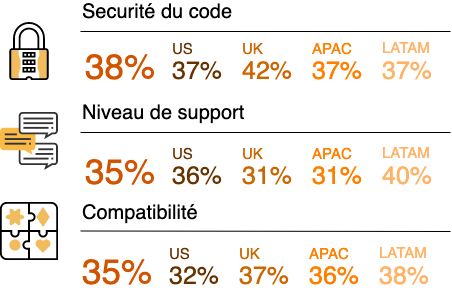
\includegraphics[scale=0.70]{./img/Barreer_os.png}
						\caption{Causes principales des réticences à l'open source}
						\caption*{\color{silver}Source: redhat.com}					
					\end{figure}										

					J'en conclu qu'à travers le hack et le piratage de produits open sources, les entreprise positionnent la sécurité de l'open source comme une inquiétude majeure.

				\paragraph{L'évolution de l'utilisation de l'open source\\}

					Beaucoup d'entreprises continuent tout de même à utiliser des logiciels propriétaires, mais cette tendance tend à diminuer sur les deux prochaines années. Ceci grâce aux nouvelles technologies provenant du \gls{web 3.0}, notemment la \gls{conteneurisation}, qui est considérée comme un brassage de produits collaboratifs open sources. De nombreuses entreprises aujourd'hui se tournent vers des solutions de conteneurisation, due à l'open source.
					
					\begin{figure}[!htb]
						\center
						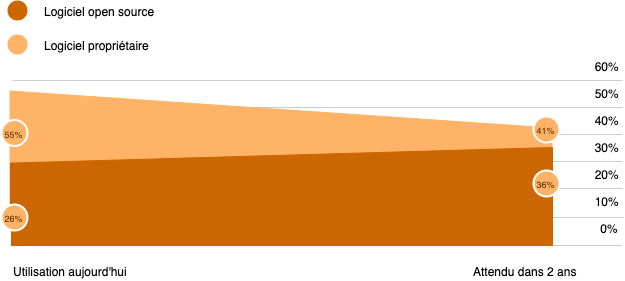
\includegraphics[scale=0.60]{./img/osinentreprise.png}
						\caption{Évolution de l'open source dans les années à suivre}
						\caption*{\color{silver}Source: redhat.com}					
					\end{figure}

					\newpage

	\section{Problématique}
		\paragraph*{}

			Je vous propose de traiter la problématique suivante :
			\begin{center}
				\begin{displayquote}
					\textbf{Comment valoriser l'open source, en tant qu'éditeur, et en faire la solution privilégiée des consommateurs ?}
				\end{displayquote}
			\end{center}

		\paragraph*{}
			
			Afin de répondre à cette problématique, je vais m'appuyer sur des hypothèses fondées sur mon vécu en entreprise mais également issues de ma réflexion personnelle dans mon métier de développeur logiciel.

	\section{Hypothèses}

		\paragraph{Promouvoir l'open source\\}

			Selon moi si les plateformes hébergeant du contenu open source et offrant la possibilité d'y contribuer mettaient plus en avant les projets open sources, par une démarche plus marketing et publicitaire à travers l'utilisation d'images et la présentation du projet par vidéo, l'open source serait plus prisé par les consommateurs et l'on constaterait plus de contributions à ces projets.

		\paragraph{L'optimisation\\}

			Si nous améliorons l'organisation de la communauté, en impliquant un peu mieux les personnes sans pour autant compliquer leur participation , nous valoriserons l'open source en le rendant plus performant.

		\paragraph{L'envie de contribuer\\}

			Si toutes les personnes liés à l'informatique était sensibilisées sur l'importance de l'open source et si l'éditeur leur donnait envie de contribuer en leur facilitant la tâche par des guides ou des moyens de s'exprimer plus facilement, l'open source serait la solution idéale à leurs yeux.

	\section{Méthodologie de travail / périmètre}
		\paragraph{Etude de l'open source}

			\subparagraph{Présentation de l'open source\\}

				Afin d'avoir un retour sur mes hypothèses, il m'est nécessaire d'avoir une meilleure vision d'ensemble de l'open source et un périmètre défini.

			\subparagraph{Les éditeurs open source\\}

				Je me positionne du côté des éditeurs, pour les diverses raisons évoquées précédemment, je souhaite donc en savoir plus sur l'éditeur, ses rôles, son périmètre d'action.

			\subparagraph{L'optimisation des ressources\\}
		
				Après avoir fait la lecture et l'analyse personnelle de plusieurs ouvrages dont 2 principaux sur lesquels je m'appuierai : 
		
				\begin{displayquote}
					\textquote{Réfléchissez et devenez riche} - Napoleon \bsc{Hill} - 1937
				\end{displayquote}
				\begin{displayquote}
					\textquote{Oser la confiance} - Bertrand \bsc{Martin} (†), Vincent \bsc{Lenhardt}, Bruno \bsc{Jarrosson} - 1996
				\end{displayquote}
		
				Je souhaite effectuer des recherches sur les moyens d'optimiser les ressources qui définissent l'open source.

			\subparagraph{Le consommateur\\}
				En étudiant le consommateur, nous verrons les besoins et activités relatives à l'open source.

			\subparagraph{Le marché de l'open source\\}
				Enfin nous verrons l'aspect économique associé à l'open source en étudiant son marché.

		\paragraph{Sur le terrain \\}
			Lors de mon étude terrain je consoliderai mes recherches dans les domaines cités précédemment pour pouvoir les confronter.

		\paragraph{L'analyse et les résultats \\}
			Je transposerai alors mes études et relevés afin de valider ou réfuter mes hypothèses et apporter une réponse acceptable à ma problématique.
\chapter{\color{burntorange}{Etat de l'art}} %20 pages

	% --------------------------------------------------%
	%     												%
	%             Présentation de l'open source			%
	%       										    %
	% --------------------------------------------------%

	\section{Présentation de l'open source} % ready to review

		\subsection{L'open source aujourd'hui}

			\subsubsection{Faire de l'open source c'est ...}

				\paragraph{Un mouvement de pensée\\}

					Le logiciel open source est une affaire de liberté. N'importe quel programme devrait être utilisable, modifiable et redistribuable. Les logiciels non libres, "propriétaire", porte atteinte à cette philosophie. Le logiciel libre n'est pas une alternative ou bien un autre business model mais une lutte pour la liberté.

					Un grand mouvement est initié par Richard \bsc{Stallman}, le père fondateur de la \acrshort{fsf} qui soulève un patrimoine extraordinaire de logiciel mis à disposition de tous. Il s'agit d'une véritable révolution pour ce mouvement de pensée profond ou la solidarité sociale et l'entraide en sont les pilliers.

				\paragraph{Un modèle de développement\\}

					L'utilisation d'un modèle de développement open source communautaire est pour Eric \bsc{Raymond} un moyen de démontrer la \textit{supériorité} des logiciels réalisés. Plus que des valeurs éthiques, c'est par la création de ce mouvement avec la fondation de l'\acrshort{osi} qu'Eric \bsc{Raymond} espère imposer l'open source. Pour certain, ceci apparaît comme une \textit{opération marketing}, pour d'autre comme Richard \bsc{Stallman}, il n'est pas permis de jeter les valeurs fondatrices notemment la \textit{liberté}. 

				\paragraph{Une dimension humaniste et un patrimoine\\}

					L'open source permet avant tout d'offrir une chance pour les informaticiens futur de ne pas repartir de zéro, ne pas ré-inventer la roue. Chaque participation de l'Humain apporte sa pierre à l'édifice.
					Selon Smile, la société leader en Europe de l'open source, seulement 10\% d'un code source est issue de notre création pour 90\% de réutilisation de code issus de système d'exploitation, \gls{framework}, et autres composants.

					C'est ici la valeur ajoutée de l'open source. L'informatique progresse essentiellement car le socle de code qui constitue notre patrimoine s'agrandit.

				\paragraph{Respecter des droits\\}

					Les programmes open source ne sont pas des programmes « sans licences » comme on l'entend parfois. C'est au contraire leur licence qui les fait open source. Ils ne sont pas non plus dans le domaine public, c'est à dire n'appartenant à personne en particulier, ou du moins exempts de droits patrimoniaux.\\
					Lorsqu'un développeur écrit un programme, il en détient les droits d'auteur, le « copyright ». Dans certains cas, ce peut être l'entreprise qui l'emploie qui en détient les droits. Et ce copyright peut être vendu, comme bien immatériel, d'une entreprise à une autre. \\

					Le détenteur du copyright est libre de définir l'utilisation qui peut être faite de son programme : 

					\begin{itemize}[label=\textbullet, font=\LARGE \color{burntorange}]
						\item Il peut le garder pour lui, en interdire l'utilisation à qui que ce soit.
						\item Il peut vendre ses droits à un tiers, personne physique ou morale.
						\item Il peut utiliser son droit d'auteur pour préciser les conditions qu'il pose à l'utilisation de son programme. Il écrit ces conditions dans les termes de la licence d'utilisation.
					\end{itemize}
				
					Il est donc important de bien assimiler la logique suivante : à la base de l'open source il y a la licence, et la licence n'existe qu'à partir du droit d'auteur.\\

					Ainsi tous les logiciels open source ont un propriétaire, ils ne sont pas « à personne », ni même « à tout le monde ». Dans certains cas, ce propriétaire peut être une fondation à but non lucratif, ou bien ce peut être une entreprise commerciale ordinaire. Il peut s'agir aussi de plusieurs coauteurs, en particulier à la suite de contributions successives.\\

					Le détenteur des droits est libre de fixer les conditions de licence, il est libre de changer de modèle même (GPL, Affero, AGPL), et il est libre d'y faire des aménagements ou exceptions, ou de diffuser à certains selon une licence, à d'autres selon une autre licence.\\

					Celui qui reçoit le programme, en revanche, n'est pas libre. Il est lié par les termes de la licence. Certes il n'a pas signé de contrat, mais la licence lui a été bien énoncée, et elle stipule qu'il n'a le droit d'utiliser le programme que sous telles et telles conditions. S'il refuse ces conditions, il n'a pas le droit d'utiliser le programme. 
					
		\subsection{Les éditeurs open source}

			\subsubsection{Zoom sur l'éditeur}

				L'éditeur, c'est celui qui détient les droits du produit, en assure le développement, la promotion, la diffusion et le support.\\
			
				La seule différence avec l'éditeur de logiciels pour l'éditeur open source est qu'il publie son produit sous licence open source. Sinon l'investissement dans le développement du produit et son marketing est le même qu'un produit propriétaire.
				Ce modèle a été élu pour permettre de briser les position acquise d'oligopoles sur le marché du logiciel.
				Il s'agit donc majoritairement de petites entreprises éditrice qui font du support et du développement du produit leur credos.
				Développer un programme open source coute (un peu) moins cher pour ces entreprises car :

				\begin{enumerate}[font=\color{burntorange}]
		 			\item Elles peuvent s'appuyer sur autant de brique que la licence de son logiciel lui permette.
		 			\item Elles bénéficient de contributions communautaire, que je détaille ultérieurement.
			 		\item Elles possèdent généralement plus de développeurs passionnés qui participent à son travail.
				\end{enumerate}

				Nous parlerons plus en détail du modèle économique des éditeurs dans la partie sur le marché de l'open source.
				Généralement, l'éditeur fait le choix de partir sur une licence dite GPL car elle présente pour eux deux avantages considérables:

				\begin{enumerate}[font=\color{burntorange}]
		 			\item Du fait de sa popularité, elle est parfaitement lisible et compréhensible ce qui la rend gage de tranparence.
		 			\item Elle empêche les autres de se faire de l'argent sur son dos car elle interdit l'intégration du produit dans un développement propriétaire.
				\end{enumerate}

			\subsubsection{L'aspect communautaire}

				L'éditeur open source a à sa disposition une communauté qui pourra l'aider non seulement dans le support sur les ressources open source qu'il utilise mais également au développement et au support de son oeuvre.

				Au sein de la communauté il est possible de distinguer deux types d'acteurs:

				\begin{description}[font=\color{burntorange}]
					\item[les développeurs indépendants: ] Qu'il s'agisse de gloire, de monté en compétence sur un domaine ou d'altruisme, il existe des développeurs qui soutiennent le développement de produit et participent au support.
					\item[Les contributeurs et entreprises contributrices: ] Certaines entreprises favorisent l'aide et autorise leurs employés à travailler une partie de leurs temps d'activité sur des projets open sources.
				\end{description}

				Parmis ces contributeurs, on retrouve beaucoup de salariés d'entreprise IT et ce pour plusieurs raisons comme:

				\begin{itemize}[label=\textbullet, font=\LARGE \color{burntorange}]
					\item Le marketing: statuer que l'on a un développeur qui travaille sur un « Grand projet » pour dorer son image et promouvoir son entreprise.
					\item La gouvernance: car cela permet d'avoir son mot à dire sur les orientations stratégiques d'un produit
					\item Le socle technique: Plus il y a de contributions à un socle de produit open source dont l'entreprise est utilisatrice, meilleur sera leur business.
					\item La maitrise du produit: Monter en compétence et proposer du support sur ce produit.
				\end{itemize}

				\paragraph{Les contributions communautaires\\}

				De manière générale, les éditeurs open source ne sont pas trop pour l'apport par le biais de la communauté, du moins sur le coeur de leur produit. Ils les acceptent car c'est dans la logique de l'open source, mais ne les encouragent guère ce qui m'apparait comme un frein à l'utilisation du plein potentiel de l'open source\\

				Lorsque le code du contributeur est accepté, il passe sous un accord spécifique signé avec l'éditeur qui dispose librement du code. Cela empêche chaque contributeurs de spécifier ses clauses de licence conduisant à un sac de noeud de licences.\\

				Afin de conserver la maitrise de leur noyau mais d'apporter l'aspect communautaire, les éditeurs utilisent un dispositif d'extensions, qui enrichit le produit indépendemment du noyau . Bien que rapidement évoqué, je détaille plus ce modèle noyau-extension dans la partie sur l'optimisation des ressources.

			\subsubsection{Les supports de l'open source}

				Le support dans le monde du logiciel, c'est la capacité à apporter de l'aide dans l'utilisation du programme et à corriger le programme le cas échéant.\\
				
				Le support peut s'adresser aux utilisateurs finaux, comme aux exploitants du programme, ou encore aux programmeurs travaillant sur le programme.\\
				
				Le déploiement de programmes pour des tâches critiques, en particulier dans des entreprises, requiert absolument un support, car le risque d'une situation de blocage est trop important, cela que ce blocage soit dû à une anomalie ou à un mauvais usage, mauvaise configuration, incompatibilité, etc.

				\paragraph{Le support de l'éditeur\\}

				Du côté des éditeurs open source (MySql, eZ Publish, OpenERP, ...), la question est différente: l'éditeur est une société commerciale et son business model est essentiellement basé sur son offre de support. Ici donc, le dispositif de support est très proche de celui des produits propriétaires. Pas identique toutefois car \textit{en parallèle, en complément} au support payant de l'éditeur, il existe souvent un support communautaire, plus ou moins vivace selon les produits.Mais le plus souvent, les corrections touchant au code ne sont assurées que par l'éditeur.\\

				Pour les nouveaux éditeurs de l'open source commercial, le support produit est le fondement du business model, il est leur raison de vivre, leur unique source de revenus. On peut donc s'attendre à un support de grande qualité.

				\paragraph{Le support de la communauté\\}

				Les produits communautaires bénéficient avant tout d'un support communautaire. C'est à dire basé sur le volontariat de développeurs impliqués, qui répondent aux questions des utilisateurs sur les mailing-lists et forums. Et basé également sur le suivi et la prise en charge des anomalies sur les plateformes de développement communautaires.\\

				Lorsque la communauté est active, comme c'est le cas autour des grands produits, ce support communautaire peut être d'une très grande efficacité, d'une très grande réactivité, très supérieur à un support commercial.\\

				Nous verrons plus tard comment améliorer cette gestion de la communauté dans la partie optimisation des ressources.

		\subsection{Le consommateur}

			\subsubsection{Qui est le consommateur ?}

			Je classifie les consommateurs en trois catégories distinctes :
			\begin{description}[font=\color{burntorange}]
				\item[Les end-users:] Ce sont les clients finaux du produit open source. Si le logiciel open source à pour vocation d'être utilisé comme tel par le grand public ou bien parmis les entreprises, on considère ces personnes comme des utilisateurs finaux ou \textit{« end-users »}. Ils utilisent le logiciel, remontent leurs besoins d'amélioration, de correctifs et de support.
				\item[Les contributeurs et la communauté:] consomme l'open source car ils y contribuent, en adaptant certains besoins du logiciel par la création d'extension, par l'aide au développement, et tout soutient qui implique l'utilisation du produit de l'éditeur.
				\item[Les autres éditeurs et prestataires:] Comme nous l'avons aperçu précedemment, une licence open source permet de bénéficier de toutes les ressources sous la même licence. Les développeurs chez les éditeurs et prestataires réalisent des aggrégats de différentes solutions open sources à laquelle ils intégrent la leur. Nous le verrons plus en détail dans la partie concernant l'intégration de solution.
			\end{description}

			Il est important de considérer que nous somme tous des consommateurs appartenants à la catégorie « end-user » car aujourd'hui, nous avons tous utilisé au moins une application, une partie de logiciel qui utilise de l'open source. Même sans en avoir conscience.

			Favoriser l'open source pour ces consommateurs c'est leur permettre une expérience plus libre dans leurs besoins. Voyons à présent quels en sont leur bénéfices.
			
			\subsubsection{Les bénéfices de l'open source pour le client}

			Meme si les solution open source ne sont pas toute gratuites, elles sont en générale moins couteuse, ce qui en fait un critère de choix essentiel aux yeux des consommateurs.

			Le produit étant ouvert, la diffusion des source tend à réduire le coût des prestations associés car la communauté est de plus en plus compétente et permet de se passer de prestations telles que le support.

			Mais au fur et à mesure que ces solutions arrivent à maturité, le moindre coût n'est plus le premier critère de choix.
			Les principaux arguments sont alors :

			\begin{itemize}[label=\textbullet, font=\LARGE \color{burntorange}]
				\item \textbf{La non-dépendance}, par rapport à un éditeur. Comme changer d'outil est souvent cher pour les entreprises, il peut être intéressant de se détacher d'un propriétaire qui souhaite garder sa « vache à lait ».
				\item \textbf{L'ouverture} des solution open source les rends plus respectueuses des standards, et plus ouvertes vers l'ajout de modules d'extension.
				\item \textbf{La pérennité}, du fait de sa diffusion, le logiciel devient un bien commun que l'on souhaite péreniser. 
				\item \textbf{Et la qualité} due au grand nombre de déploiements et donc de retours d'expérience, mais aussi le modèle de développement et l'intégration de composants de haut niveau, permet de dépasser les logiciels propriétaires.
			\end{itemize}

			A ceci s'ajoute le plaisir d'utiliser des programmes dont on peut acquérir la totale maîtrise, sans barrière ni technique ni juridique.

		\subsection{Où trouver de l'open source ?} 

			Que l'on souhaite démarrer son projet open source ou contribuer au patrimoine du Logiciel Libre, de nombreuses plateforme et espace web permettent le stockage et la redistribution de ces projet open sources.

			\paragraph{Plateforme de dépot de code}

				\subparagraph{Github\\}
				La plateforme «open source» par excellence centralisant le code source des plus grandes entreprises du monde: Google, Microsoft, Netflix, Facebook, Apple entre autres.

				\begin{figure}[h]
					\center
					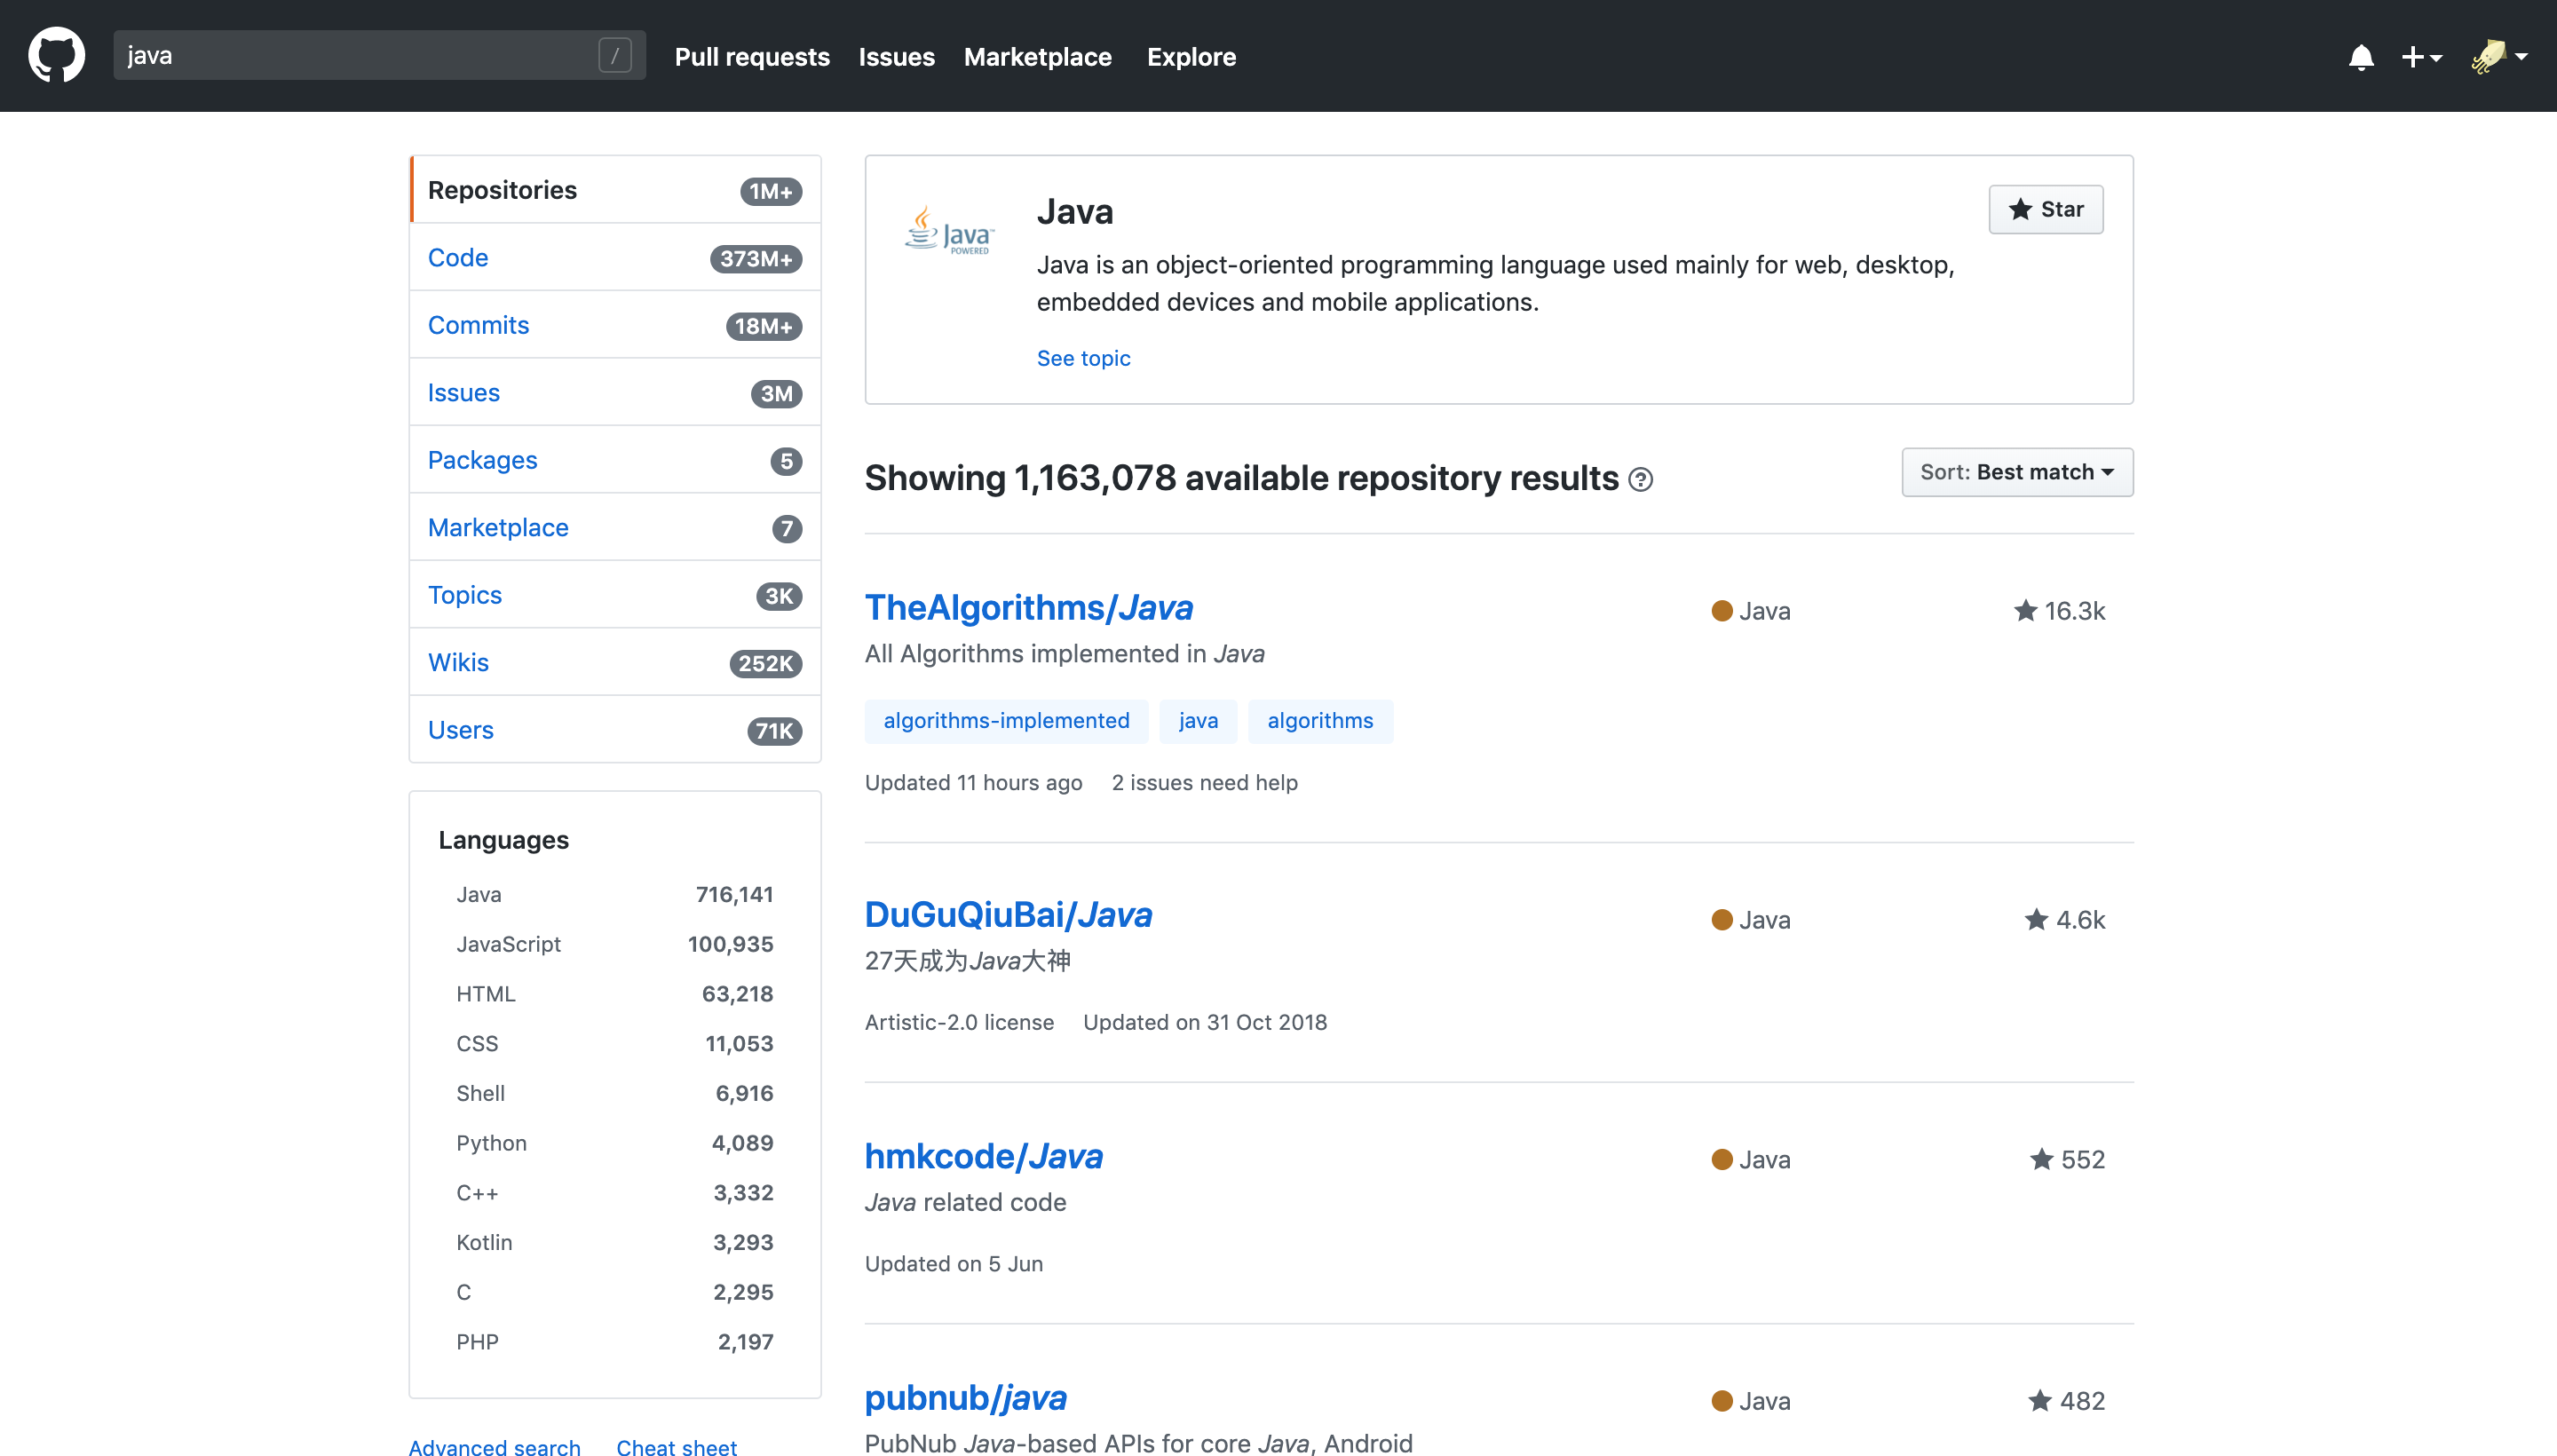
\includegraphics[scale=0.28]{./img/gh_os}
					\caption{Interface de github}					
				\end{figure}
				\newpage
			
				\subparagraph{Bitbucket\\}
				Très similaire à GitHub, Bitbucket est un hébergeur de code source libre qui permet à chacun de s’intéresser à des solutions libres.
				

			\paragraph{Plateforme de promotion de projet}

				\subparagraph{Google Open Source\\}

				Avec plus de 2000 projets libres sous sa tutelle, Google Open Source est un incubateur des nouveaux projets libres sur le marché.
				La plateforme est simple, rechercher un projet comme une recherche google, ou attendre la présentation de différents projets et laisser la magie opérer 

				\begin{figure}[h]
					\center
					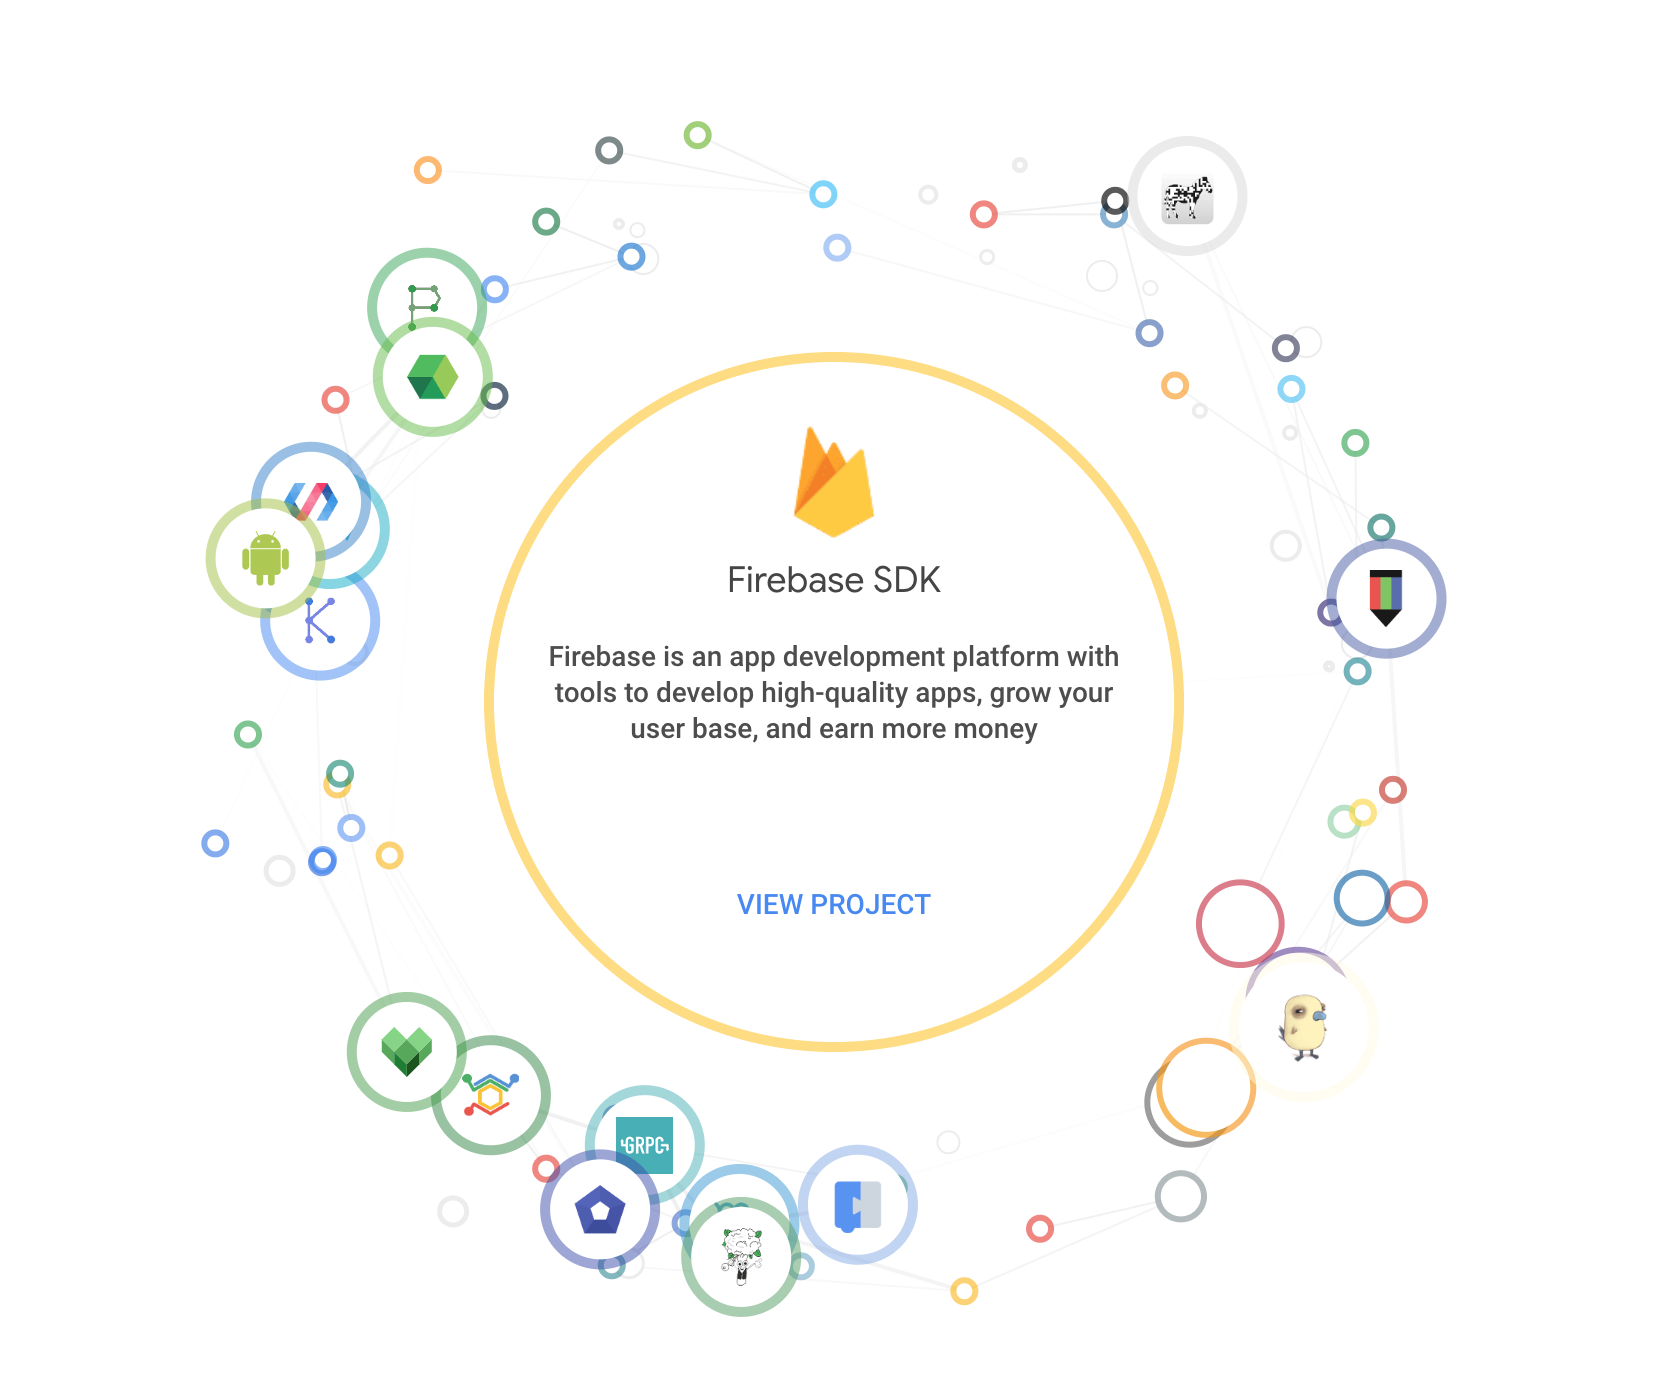
\includegraphics[scale=0.35]{./img/google_os}
					\caption{Interface de google open source}					
				\end{figure}

				\subparagraph{Github Explore\\}
				L'interface simplifié pour démarrer et trouver un projet open source auquel contribuer.

				\begin{figure}[h]
					\center
					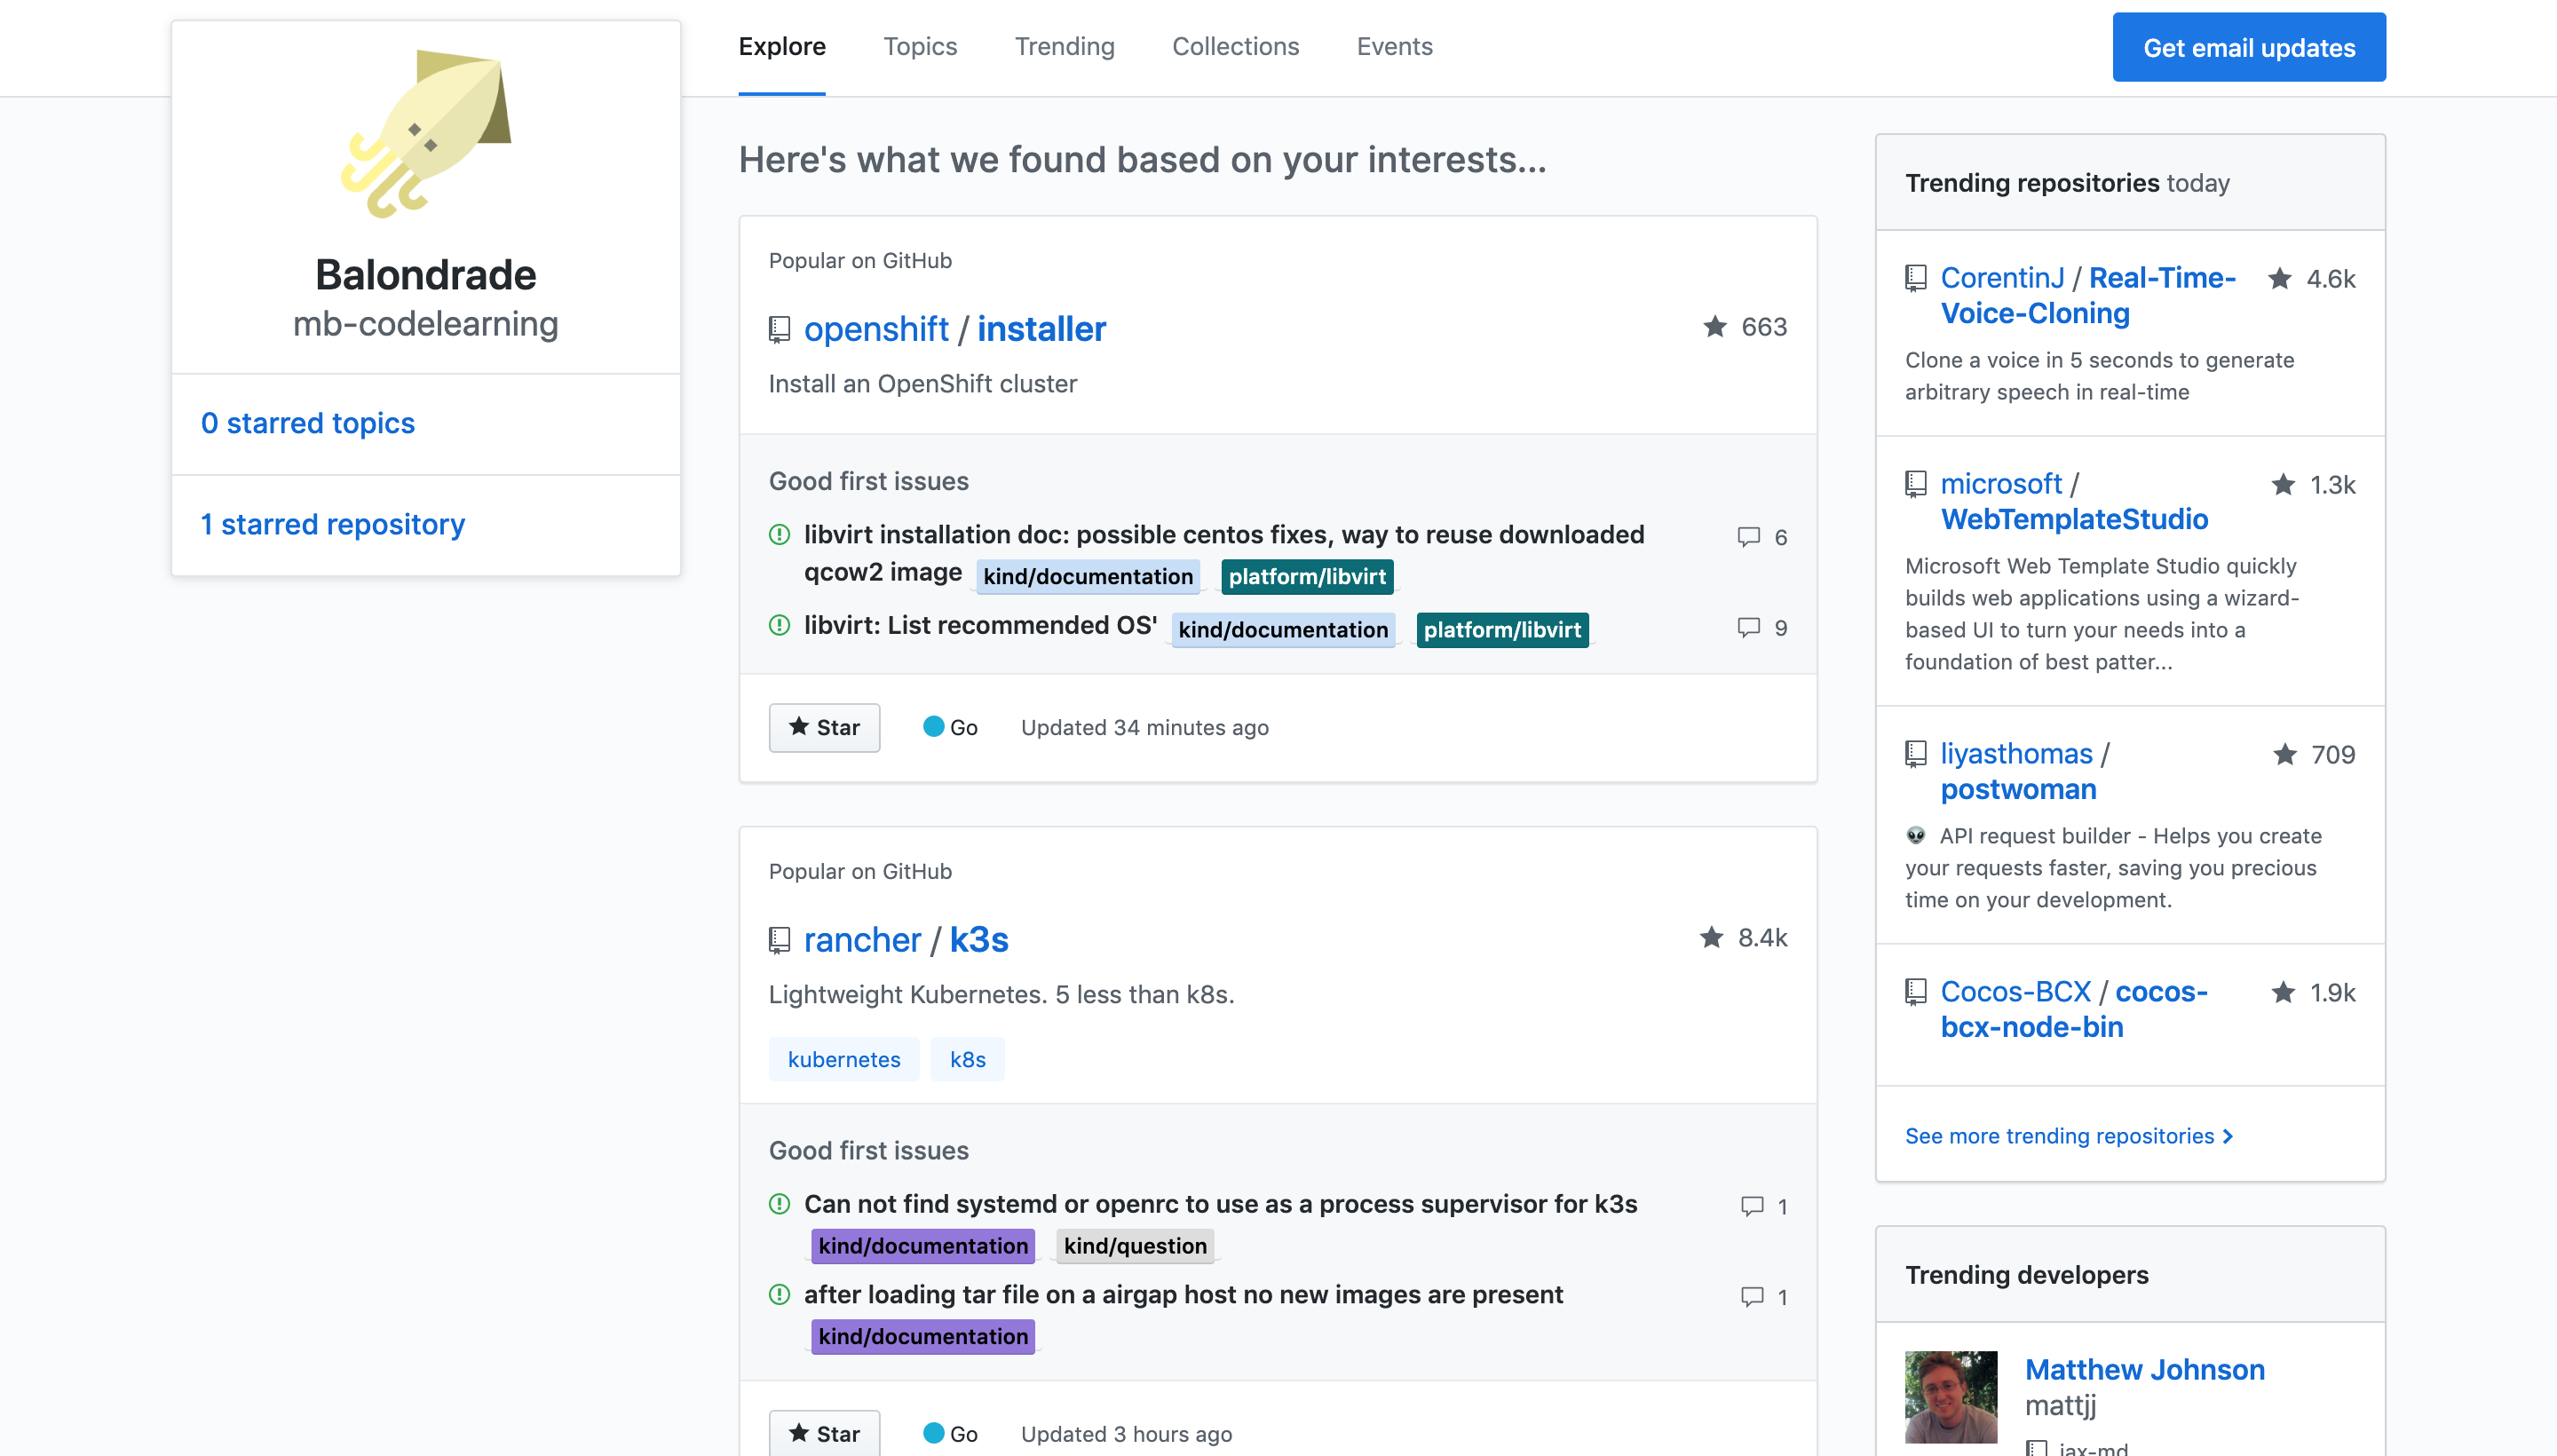
\includegraphics[scale=0.30]{./img/gh_explore_os}
					\caption{Interface de github explore}					
				\end{figure}

				\subparagraph{Open source friday\\}
				Github propose comme date de rendez-vous tout les vendredi pour contribuer chaque semaines à enrichir le logiciel libre pour les curieux et les plus passionnés.

				\subparagraph{24 pull request\\}

				Chaque année pour la période de Noël, 24 Pull Request organise un moment de développement logiciel sur de l'open source avec comme objectif de remercier les éditeurs et leurs projets qui nous aident tant.
				En 2018, \textbf{1364} contributeurs ont participés sur \textbf{3321} différents projets open sources.

				\subparagraph{Code triage\\}

				La plateforme CodeTriage est non seulement utile pour trouver son projet et démarrer rapidement dessus mais nous envois également un mail quotidien pour nous soutenir et nous rappeler nos engagements.

				\subparagraph{Contributor ninja\\}

				Ici plus qu'un évenement c'est une plateforme avec une interface rapide, pour contribuer très rapidement (tel un ninja!) à n'importe quel projets selon le langage de prédilection du contributeur potentiel.

				\begin{figure}[h]
					\center
					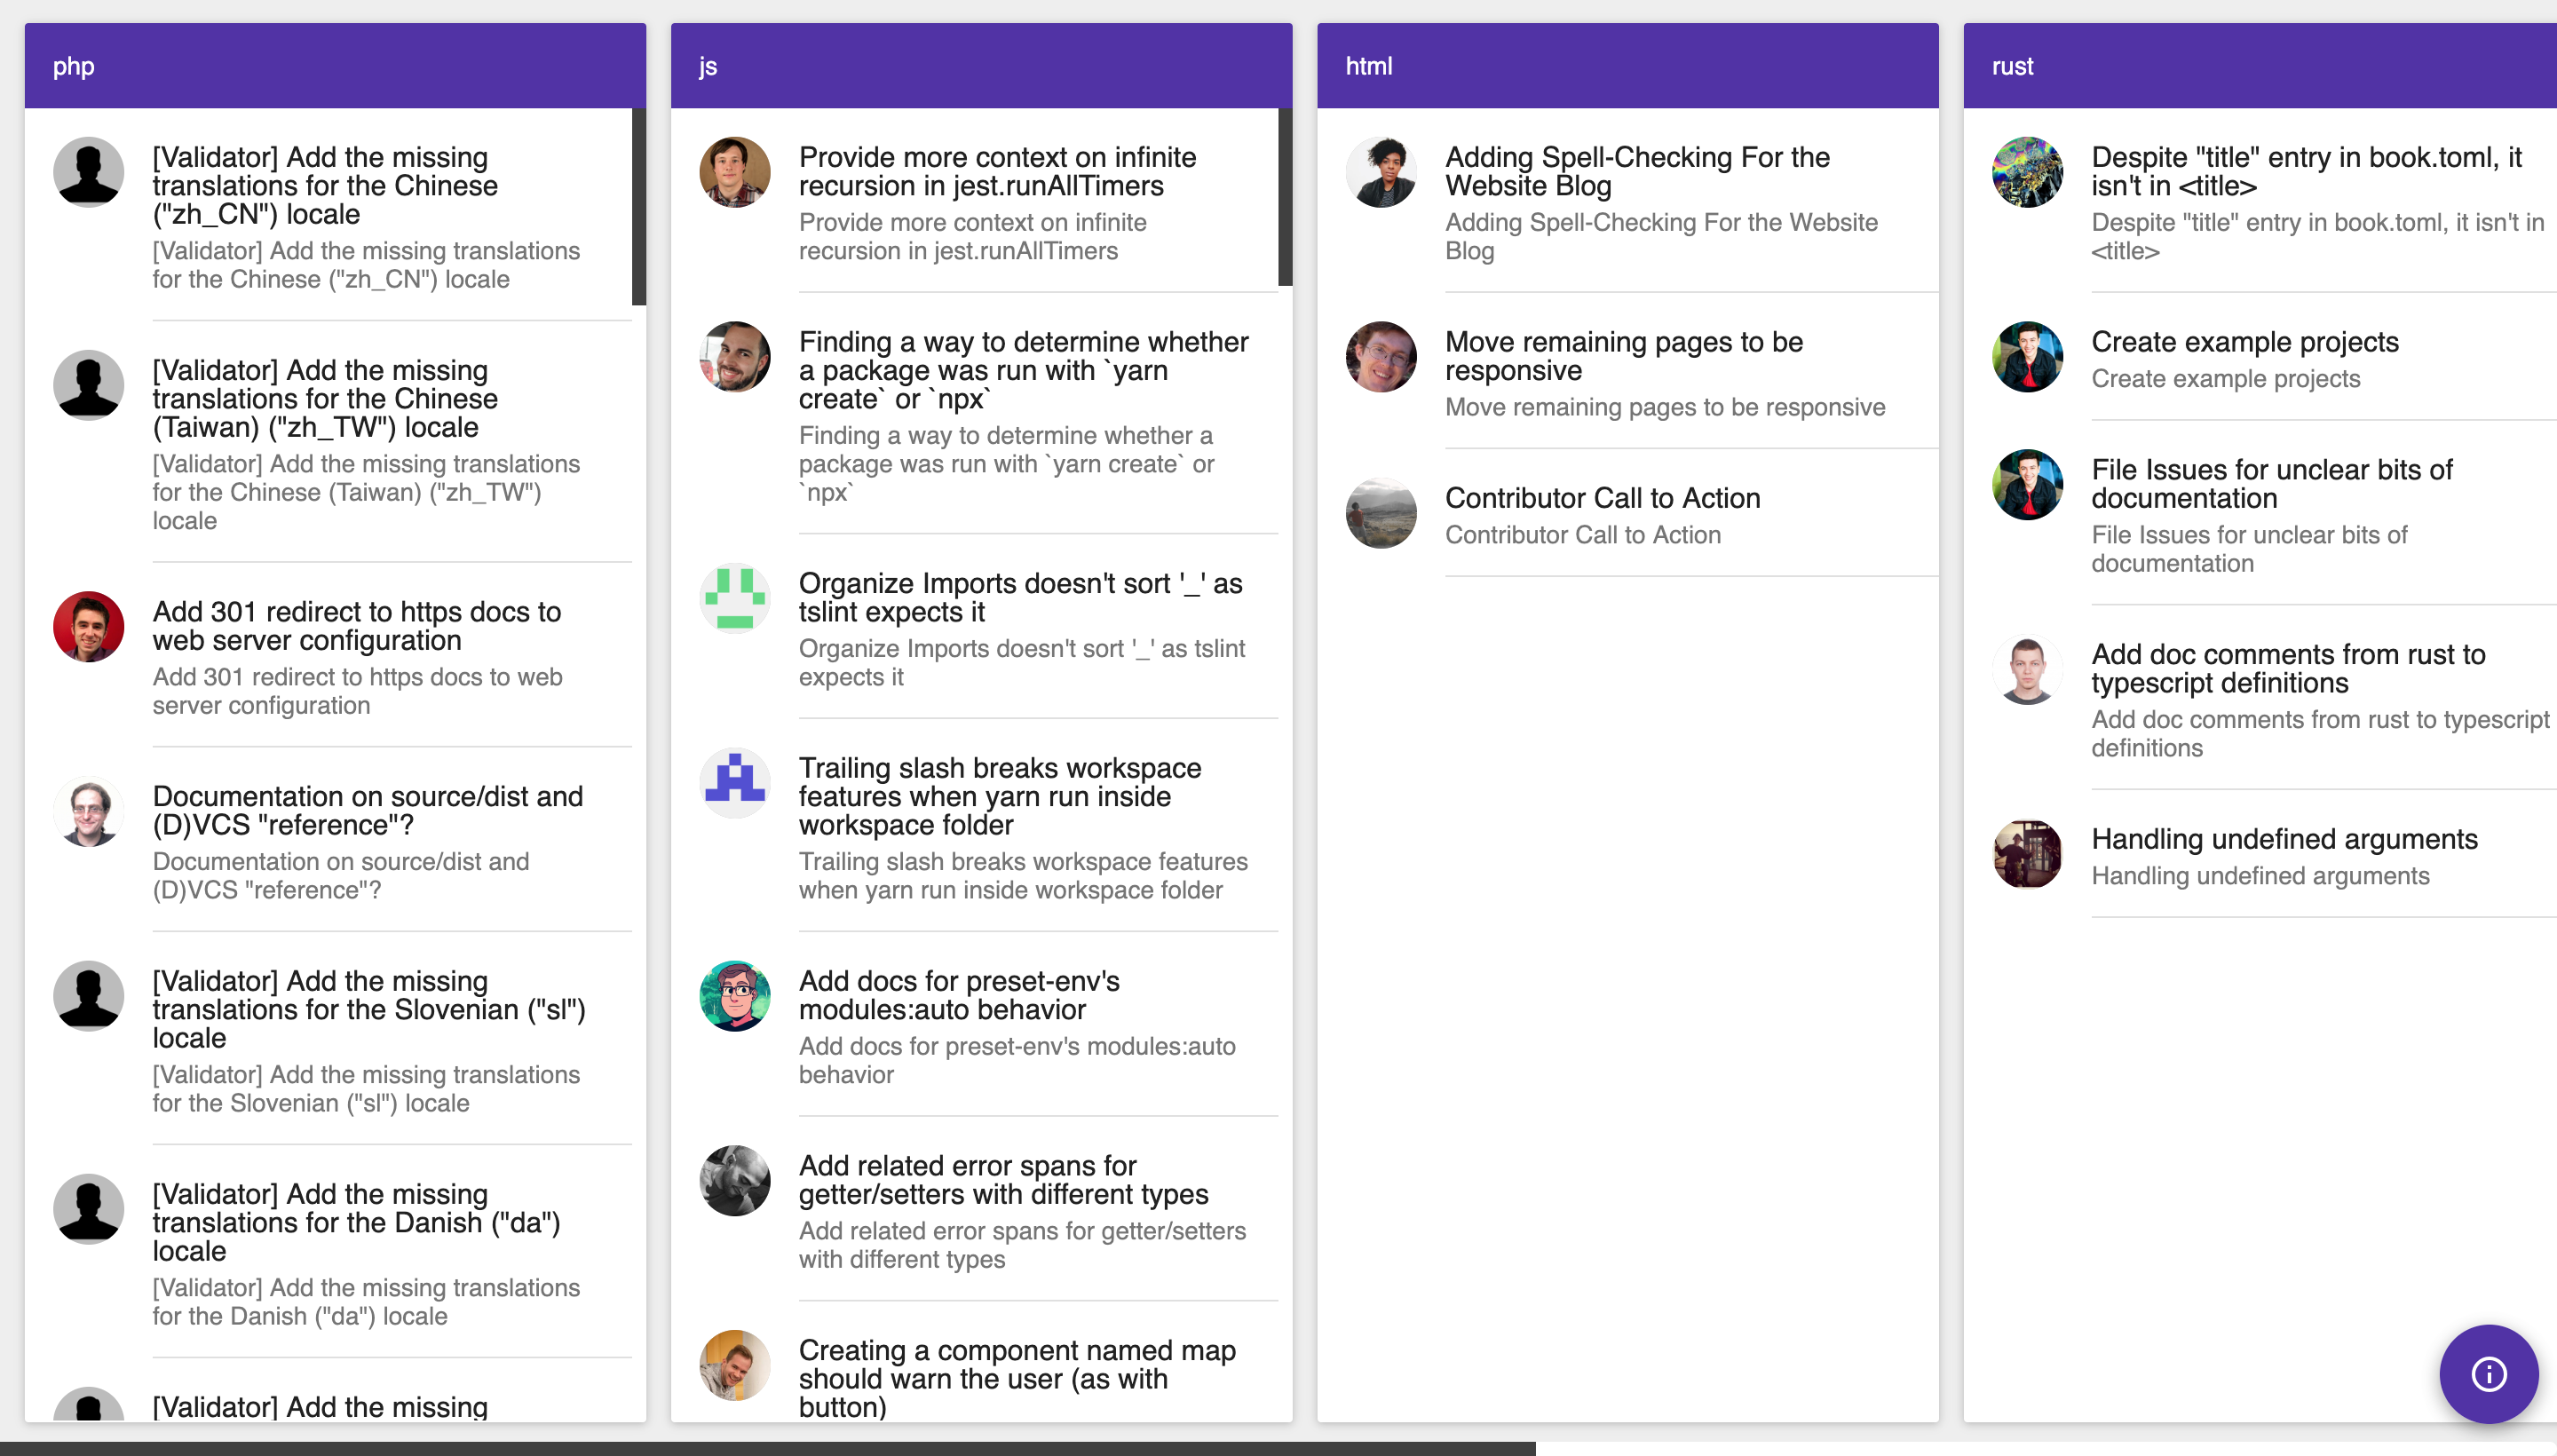
\includegraphics[scale=0.30]{./img/ninja_os}
					\caption{Interface de contributor ninja}					
				\end{figure}

				\subparagraph{Up for grabs}

				Pour vaincre toute forme de procrastination et la peur de faire le premier pas (qui handicape si souvent l'homme), up for grabs permet de rapidement trouver la bonne chaussure à son pied et se lancer dans la contribution à l'open source. Le processus est simple :

				\begin{itemize}[label=\textbullet, font=\LARGE \color{burntorange}]
					\item Lire les quelques ligne du guide de contribution
					\item Installer le projet localement
					\item Laisser un message sur la tâche que l'on s'apprête à faire
					\item Se lançer dans le travail !
				\end{itemize}

				\subparagraph{First Timers Only}

				On peut être pris au dépourvu lorsque l'on s'aperçoit que l'open source est un monde bien vaste que l'on ignorait. Pour celà, First Timers Only nous donne les clés pour débuter l'aventure dans l'open source en tant que contributeur.
		
		\paragraph{Pour conclure\\}

			L’open source est donc un mouvement important. Il apporte des valeurs de liberté, solidarité mais aussi des bénéfices tant pour les citoyens que pour les entreprises. 
		
	% --------------------------------------------------%
	%     												%
	%             Optimisation des ressources			%
	%       										    %
	% --------------------------------------------------%
	\section{Optimisation des ressources} % in progress

		\paragraph{Concept de l'optimisation\\}

	 		Le succès d'un projet open source dépend pour beaucoup de leur code, mais pas uniquement. De leur concept, de leur capacité à faire connaître le projet, à faire naître une communauté afin d'assurer la pérennité de leur aventure.

		\subsection{Le cerveau collectif}
			\paragraph{Introduction au cerveau collectif\\}

				A travers l'ouvrage de Napoleon \bsc{Hill}, intitulé \emph{« Réflechissez et devenez riche »}, on retrouve plusieurs fois la notion de cerveau collectif.

				L'élaboration d'un cerveau collectif constitue à regrouper des membres partageant les mêmes intérêt et passions ou du moins complémentaire.
				Chaque personnes veillent à maintenir un climat de confiance au sein du cerveau collectif.
				Au sein du cerveau collectif, l'intérêt est que chaque membre possède sa connaissance, son domaine particulier. 
				Napoleon \bsc{Hill} dans son oeuvre traite de personne instruite. Il définit une personne instruite, tout personne qui sans léser les intérêt d'autrui sait obtenir ce qu'elle veut.

				\subparagraph{Être instruit\\}

					Quand l'on sait que Henry \bsc{Ford} n'est allé à l'école que jusqu'à ses 6 ans. Malgré cela on peut qualifier cet homme d'instruit. Il fût traité de pacifiste ignorant pendant la première guerre mondiale par un journaliste. Afin de prouver son esprit inculte, les avocats des journalistes lui posèrent des questions innatendues sur des sujets variés. Face à tant de colles, celui-ci répondit:

					\begin{quote}
					« Permettez moi de vous rappeler que j'ai dans mon bureau une rangée de boutons électriques. Il me suffit d'appuyer sur l'un d'eux pour appeler un homme capable de répondre à n'importe quelle question relative à l'affaire dont je m'occupe personnellement(...), pourquoi je devrais avoir la cervelle farcie de culture générale alors que je suis entouré de collaborateur qui suppléent à toute lacune ou défaillance de ma part.»
					\end{quote}

			L'intérêt de vous partager cela est de vous faire réagir sur ce concept que l'on essaye tant d'inculquer à notre époque. La multi-compétence. A quoi bon souhaiter être bon dans une multitude de domaine, quand l'on peut être excellent voire une référance dans l'un des domaines qui nous siet tant.

			C'est sur ce principe que se base le fondement du cerveau collectif. \textbf{Utiliser le plein pouvoir de la connaissance de personnes} si compétentes dans un domaine qu'il serait une perte de temps de chercher à les égaler.
			Egalement, je rajouterai que le cerveau collectif se veut complémentaire et que l'intéraction entre les divers membres permet d'aller encore plus loin ensemble mais surtout indépendemment.
			Ainsi, on peut définir un cerveau collectif par les concepts suivants : \\

			\begin{itemize}[label=\textbullet, font=\LARGE \color{burntorange}]
				\item Avoir un même idéal, but commun et être sur la même longueur d'onde.
				\item Un climat de confiance règne au sein de l'équipage.
				\item Chacun sa compétence qu'il améliore au fil du temps.
				\item Utiliser en collaboration les compétences de chaque membre dans leur domaine afin d'en résulter un plein pouvoir permettant de mener un projet à l'excellence.
			\end{itemize}

			\begin{quote}
			 « Si deux esprits travaillent ensemble, ils libèrent une troisième force invisible et intangible qui est semblable à un troisième esprit » - Napoleon \bsc{Hill} - \emph{Réflechissez et devenez riche}
			\end{quote}

			Imaginez si ce concept s'applique à l'ensemble de la communauté. C'est avec ce principe que nait mon idée d'optimiser la communauté d'un projet open source et le rendre incontournable.

			Le cerveau collectif à déja fait ses preuves pour nombres de personnes. Napoleon Hill décrit le succès du célèbre industriel Andrew \bsc{Carnegie} dont je vous invite à lire sa bibliographie. Il a utilisé le cerveau collectif avec son équipe d'une cinquantaine de personne dans l'industrie de l'acier.

			\paragraph{Application du cerveau collectif au sein de la communauté}

			Bien évidemment avant de pouvoir appliquer ce concept il faut le faire accepter par les membres, qu'ils aient le même esprit de travail, ambition ou qu'ils puissent comprendre et se tourner vers ce mode de pensée.

				\subparagraph{Choisir les membres du cerveau collectif\\}

					Bien choisir son équipe est l'élement prédominant dans tout projet. Je pars du principe que l'on souhaite monter une communauté qui nous aidera à travailler sur notre projet. Il me semble alors essentiel avant de fonder le projet, de rechercher les membres essentiels qui composeront le cerveau collectif qui menera à bien le projet.

					L'idée de démarrer dès que possible son projet est certe une direction tentante pour très vite faire contribuer des membres mais penser dès la conception du projet à monter le coeur du cerveau collectif permet de gagner un temps d'avance sur les étapes futures. Egalement celà renforcera les décision prises afin que le projet se stabilise le plus rapidement possible.

					Alors avant de démarrer sur les chapeaux de roue, prenons le temps dès que l'on souhaite se lancer dans un projet, de trouver et d'impliquer les ressources humaines essentielles nécessaire à la construction de celui-ci. 

				\subparagraph{Choisir un support de communication adapté\\}

					L'outil de communication avec le cerveau collectif sera la principale source d'inspiration, de compte rendu, de retour et d'évolution du projet.
					Lorsque l'on souhaite se lancer en tant qu'éditeur d'un logiciel open source, il est important de veiller à mettre en place un outil de communication propre et clair sur lequel les décisions seront inscrite durablement.
					Savoir prendre des décisions précises sur lesquel nous ne revenons pas fait partis des qualités essentielle d'un dirigeant.

					Chaque membre du cerveau collectif est donc responsable des directions qu'il souhaite faire prendre au projet, à l'équipe, à la communauté et l'on attendra de lui qu'il ne devienne pas une girouette car il représente une partie importante du projet.

				\subparagraph{Gestion du cerveau collectif\\}

					Le cerveau collectif est alors composé des membres du coeur du produit, le « noyau » que je détaille dans la partie sur le modèle noyau-extension et de la communauté qui eux constituent les équipes qui gravitent autour du projet et réalisent les extensions.

					Gérer la communauté par domaine de connaissance ou métier permet de catégoriser et focaliser sur les contributions à apporter.
					Un cerveau collectif central et de multiple cerveaux collectifs qui gravitent autour du noyau permettront de maintenir le cadre d'évolution nécessaire à ce mode de pensée.

				\subparagraph{La communication au coeur de la stratégie\\}

					Et maintenant quoi ? On a un cerveau collectif, on a choisi les membres, on a respecté leur domaines de prédilection, mis en relation ... Mais ou est la stratégie pour développer et déployer notre projet ?

					La gestion de projet inhérente à l'édition d'un logiciel est un standard que je ne développe pas ici (méthodologie agile, gestion d'entreprise) mais l'on pourra compléter ceci avec l'ouvrage « Oser la confiance » comme nous le verrons dans la partie « Eveiller sa communauté » .

		\subsection{Rendre le libre populaire}

			\paragraph{Pareto revisité\\}

				Une étude sur la participation de développeur et le code total rédigé rapporte que si l'on prend un projet ou 200 programmeurs participent, seulement, 10 d'entre eux ont écris 50\% du code. C'est donc la preuve d'un investissement mal répartis généralement dans la programmation logicielle. Il faut donc veiller à \textbf{mettre en place une implication des participant au code} et plus largement au projet.

			\subsubsection{L'enseignement du logiciel libre}

				Comme mentionné dans l'introduction de ce document, le logiciel libre me semble pas suffisemment enseigné.\\

				\textbf{Qu'est-ce que j'entend par enseigner le logiciel libre ?}

				\paragraph{Susciter l'intérer du libre\\}

					Enseigner un logiciel libre par la mise en place d'efforts spécifiques à celui-ci. 

					Je retrouve dans le livre blanc «Point de vue sur l'open source » de Smile mon hypothèse concernant le manque d'enseignement de l'open source. Ce n'est pas en utilisant sans le savoir de l'open source ou en cherchant spécifiquement à remplacer tout logiciel propriétaire par du libre que l'on enseigne l'open source. Il est nécessaire d'\textbf{expliquer les mécanismes} liés à l'open source, de prendre le temps d'\textbf{informer sur toute l'importance} de ce qui gravite autour de l'open source.\\
					Ceci afin de permettre à des centaines de programmeur éparpillé sur la planète à coopérer de façon cohérente sur la réalisation des millions de lignes de code.\\

					Celà passe également, selon moi, par la \textbf{mise en relation des étudiants avec les communautés de développeur}.

				\paragraph{Améliorer la recherche sur l'open source\\}

					Il est nécessaire d'encourager la recherche, comme le souligne Smile dans son livre blanc «Comprendre l'open source», qui se développe autour des logiciels libres et \textbf{fournir des outils nouveaux} pour accompagner leur essor.\\

					Les plateformes distribuant l'open source sont à première vue trop réservée à la communauté de développeurs, des « Nerds » qui développent la nuit.

					Des spécificité métier, tant dans le juridique et l'architecture logicielle pourrait se dégager afin de veiller au bon respect du libre.

				\paragraph{Un gisement d'emplois futur\\}

					Tant par ses valeurs humanistes que par la contribution au patrimoine de l'humanité, l'open source doit être vue comme un bien commun qu'il faut cultiver en commun.\\
					
					Tout autant que l'art qui est exposé dans de nombreux musée que l'on rends accessibles de temps en temps gratuitement pour contribuer à la culture de l'homme, \textbf{l'open source devrait être considéré de même}.\\

					Au coeur de l'activité industrielle encore méconnu, l'open source c'est 4,46 Md d' \euro{} de \acrshort{ca} révèle l'enquête du \acrfull{cnll}, en 2017. 4000 emplois nets ont été estimée d'ici 2020. La France est le leader Européen de l'open source. Et pourtant, le système éducatif actuel ne perçoit pas ce gisement. 

		\subsection{Le modèle noyau-extension, tout un écosystème}
			
			 Dans ce schéma de développement, connu pour déployer son activité open source, on distingue le noyau du produit, sous la responsabilité de l'éditeur, et les extensions, réalisées par la communauté.

				Les principes de séparation sont les suivants:

				\begin{itemize}[label=\textbullet, font=\LARGE \color{burntorange}]
					\item Le noyau doit être d'une grande robustesse, il est certifié par l'éditeur, les contributions externes y sont rares
					\item L'inferface entre le noyau et les extensions est bien documentée et stable, c'est à dire qu'un changement de version du noyau n'implique pas, du moins le plus souvent, un changement de version des extensions.	
					\item L'éditeur stimule la réalisation d'extensions, car elles donnent de la valeur à son produit et témoignent aussi de l'existence d'une communauté, en soi un gage de pérennité.
				\end{itemize}

				Ce \textbf{modèle noyau-extensions est celui qui réalise le meilleur point d'équilibre} entre les rôles respectifs de l'éditeur et de la communauté, réunissant la garantie et l'engagement de l'éditeur avec le dynamisme et l'énorme capacité de développement de la communauté.

				\begin{figure}[h]
					\center
					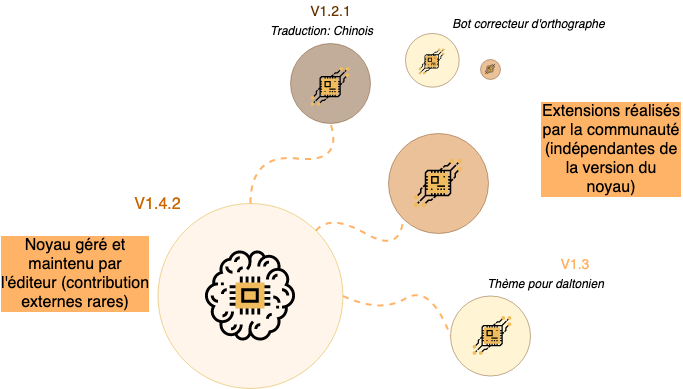
\includegraphics[scale=0.60]{./img/noyauextension_os.png}
					\caption{Représentation du modèle noyau/extension}					
				\end{figure}

				Ce modèle d'architecture présente plusieurs avantages:

				\begin{itemize}[label=\textbullet, font=\LARGE \color{burntorange}]
					\item Ne pas faire grossir inutilement un programme en se concentrant sur l'essentiel du business et de sa fonctionnalité.
					\item Jouer sur l'aspect modulable et simple du logiciel et concurrencer les logiciels propriétaires qui, sous pressions, rajoutent de plus en plus de fonctionnalités sur leur logiciel jusqu'à le rendre trop lourd .
					\item Déjouer la concurrence sur le marché, car la communauté se concentre sur la création et l' amélioration perpetuelle des extensions. Donnant un coup de neuf tout les jours.
					\item Eviter de destabiliser son logiciel car les fonctionnalités peuvent être ajouté sous forme de modules.
				\end{itemize}

				Le modèle noyau-extension permet de tracer cette frontière entre l'éditeur et la communauté tout en s'assurant que la communauté trouve sa place au sein du produit et que chacun puisse répondre à son besoin.

				Pour favoriser la mise en place et le maintient du modèle noyau-extension, l'éditeur peux \textbf{mettre généralement en place une plateforme pour accueillir ces extensions} afin d'avoir une meilleur visibilité, classer par popularité, trier selon les besoins et de rendre gloire aux auteurs de ces extensions.
			
		\subsection{Eveiller sa communauté}

			Afin de faire naitre et grandir sa propre communauté autour de son produit open source, il existe déjà quelques points clés souligné dans le livre blanc « comprendre l'open source » de Smile:

			\begin{itemize}[label=\textbullet, font=\LARGE \color{burntorange}]
				\item Semer la graine en mettant en ligne son code source. Être patient vis à vis de l'épanouissement de la communauté qui va prendre racine. Celà ne prendra pas quelques jours mais est un travail de longue halaine.
				\item Être transparent tant dans son projet et ses orientation que dans la gouvernance du projet.
				\item Choisir et décréter son support d'échange avec la communauté. Afin de centraliser la communauté sur ses outils.
				\item Instaurer sa politique de l'open source en proposant un modèle noyau-extension, celui qui fonctionne pour le mieux. Bien préciser quels sont les aspects que l'on veut retrouver dans notre vision open source.
				\item Inspirer des valeurs: le logiciel que l'on va construire n'a pas de but lucratif ou du moins il est moindre.Ceci aide à construire la communauté plus facilement car elle n'aura pas l'idée qu'on génère de l'argent sur son dos. On aspire à aider, changer le monde. Il faudra trouver l'idée d'une mission que les gens adoptent.
			\end{itemize}

			Le respect de ces standards permet d'instaurer la communauté au projet. Pour compléter ces bonnes pratiques, j'y ajoute la notion de gestion de la communauté appuyé par les propos tiré du livre « Oser la confiance » qui sont les suivants :

			\paragraph{Les valeurs}

			La mission que doit relever l'éditeur à travers son projet open source n'est pas anodine. Les valeurs qu'elle représente peuvent apporter le comportement idéal attendu des contributeur. Je souhaite donc \textbf{mettre en avant lors de la présentation de son projet, les valeurs représentées}.

			Dans l'ouvrage « Osez la confiance», une entreprise de construction navale est sur la faillite, le nouveau PDG, Bertrand \bsc{Martin} leur indique à défaut de solution qui marche avec un grand succès pour autant qu'elle n'était pas vraiment salvatrice et il témoigne :
			\begin{quote}
			\emph{« C'est parce que le personnel le voulait, qu'il avait pu s'approprier le projet, qu'il en comprenait les enjeux, que nous avons opéré avec le maximum d'efficacité»}
			\end{quote}

			\paragraph{Mettre en confiance}

			Vincent \bsc{Lenhardt} dans son livre nous confie le vrai pouvoir de la confiance, il emplois le mot \emph{empowered} qui définie clairement l'acteur d'un projet à qui l'on attribue toute confiance et dont on apporte toute ressource et aide nécessaire donne alors le meilleur de lui-même.

			Il y a donc une attitude à rechercher chez l'éditeur c'est la confiance en ses contributeurs. \textbf{Apprendre à faire confiance en sa communauté} en leur confiant des tâches essentielles, avec des enjeux dont ils ont pleinement conscience permet de dépasser ses limites pour atteindre les sommets.

			C'est ce qui a permis de relever l'entreprise de chantier naval de Bertrand \bsc{Martin}.

			\paragraph{Donner l'exemple}

			L'éditeur se doit de faire partie des élements contributeurs, se mettre non au dessus mais dans le bocal permet à chacun de se responsabiliser mais également de comprendre que l'on est une force selon le dicton « L'union fait la force». Dans oser la confiance, ce principe est bien détaillé. Vincent \bsc{Lenhardt}, analyse celà en concluant que le pouvoir et l'initiative sera entre le mains des acteurs ce qui les poussera à mettre en oeuvre les décisions. On ne recherche plus forcément la compétence de l'éditeur, ni de donner les solution mais de \textbf{déléguer et faire partie du groupe} afin d'améliorer la responsabilité des acteurs.

	% --------------------------------------------------%
	%     												%
	%              Etude du consommateur				%
	%       										    %
	% --------------------------------------------------%
	\section{Etude du consommateur} % in progress

		\subsection{le choix du consommateur}

			\paragraph{L'activité d'un projet}

			Afin d'établir un choix de solution pérenne, le consommateur va s'intérroger sur l'historique du projet et les orientations de celui-ci si il provient d'un « \gls{fork} » ou si un fork est fortement probable comme le souligne la société OpenDsi dans son article de blog intitulé « Comment choisir un logiciel libre ou open source ».
			Il pourra alors s'orienter vers toute sources d'informations disponible : blog, article, forum de discussion et liste de diffusion des activités lié à ce projet. Il peut être également intéressant de faire attention au nombre de contributeur au projet car il peut y avoir certaines incohérences autour d'un projet massivement adopté et le nombre de développeur qui le portent.

			\paragraph{La nature des contributions}

			Dans certain domaine, notemment dans celui de l'industrie, un projet open source peut fortement dépendre des contributions d'une entreprise et non d'une communauté. Ceci peut prendre différentes tournures, le projet peut partir vers un modèle propriétaire au bout d'un certain temps. Prendre des décisions qui arrangent l'entreprise en question et qui sera pénalisant pour l'utilisateur final. 

			Ainsi le consommateur sera davantage \textbf{rassuré par le nombre de contributeurs et la diversité de ceux-ci}, signe d'indépendance et de pérennité du projet.

			\paragraph{Les droits inhérents de la licence}

			En fonction du besoin du consommateur comme je vous l'ai présenté à plusieurs reprise, les licences vont permettre la ré-utilisation, la commercialisation et bien d'autres actions au projet. Le choix d'un logiciel open source se fait donc également entre la \textbf{cohérence du besoin et des idées du consommateur et les permissions accordées} à celui-ci.

		\subsection{L'expérience des consommateurs}

			Github a lancé une étude auprès de nombreux dépot de code et de la communauté qui gravite autour. C'est plus de 3800 projets open source et plus de 500 réponses qu'ils ont réussis à obtenir les conclusions suivantes:

			\paragraph{Le retour des consommateurs \\}

				Beaucoup de critiques font rages auprès des consommateurs et « pilleurs » de l'open source car ils laisseraient sans retour les éditeurs. C'est ce que critique l'article « Les logiciels libres meurent lentement sans contributions » de Framasoft, une société éditrice de solution libre. Malgré la liberté prônnée depuis le début, les éditeurs du logiciel libre s'attendent à des retours de la part des consommateurs et utilisateurs finaux. Egalement, les propositions de correction ou d'amélioration sont des retours apréciable du consommateur.
				Cette contribution permet aux éditeur de progresser et de s'adapter au marché et à la demande.
				Ainsi il s'agit d'une notion à prendre en compte dans l'optimisation de la communication avec les consommateurs. Il est possible \textbf{d'intégrer un module sur la plateforme de promotion qui facilitera les retours d'informations et critiques à l'éditeur}. 

			\paragraph{Les problèmes rencontrés par les consommateurs\\}

				Les consommateurs recensent de nombreux problèmes que l'on retrouve dans l'open source et qui peuvent être un frein à son utilisation. Lors d'une étude réalisé par github, il ressort que la documentation et le support sont essentiel auprès des consommateurs auquel je suggère de faire principalement attention. 

				\begin{figure}[h]
					\center
					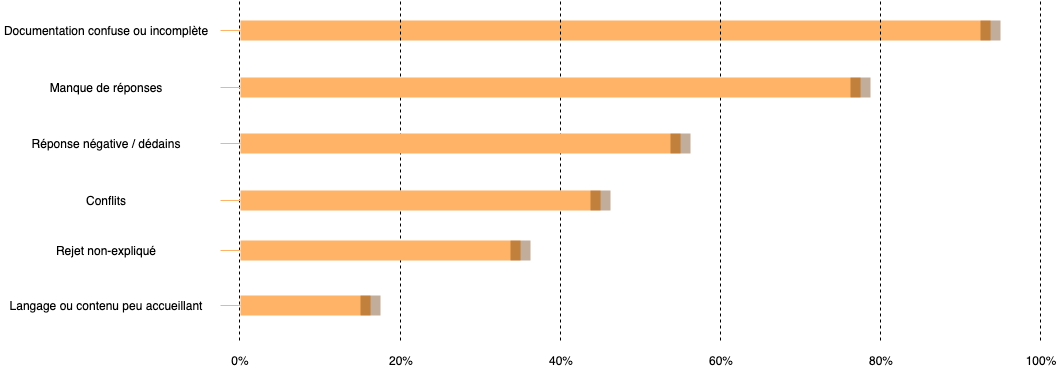
\includegraphics[scale=0.50]{./img/pb_os.png}
					\caption{Problèmes rencontrés dans l'open source par les utilisateurs}
   					\caption*{\color{silver}Source: opensourcesurvey.org}
				\end{figure}
				\clearpage

			\paragraph{Un climat néfaste ?\\}

				Au sein de projet open source du au fait d'une communauté décentralisé, virtuelle et des enjeux, nous pouvons retrouver de nombreuses violences dans les communication entres consommateur et éditeurs. Le \textbf{respect dans la communication et la bienveillance} sont des facteurs essentiels pour la satisfaction client et donc croître le nombre d'utilisateurs.

				\begin{figure}[h]
					\center
					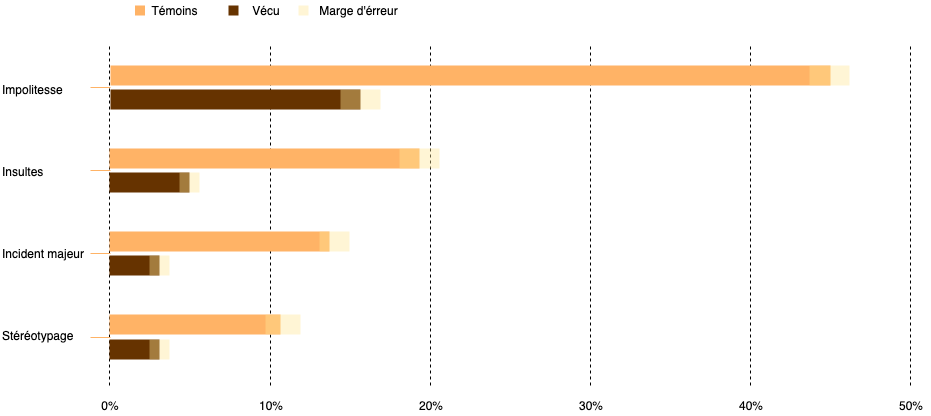
\includegraphics[scale=0.50]{./img/ng_behaviour_os.png}
					\caption{Comportement néfaste dans l'open source}
   					\caption*{\color{silver}Source: opensourcesurvey.org}
				\end{figure}

			\paragraph{Ce qui est regardé dans le choix d'un logiciel open source\\}

				Sur les utilisateurs intérrogés, un classement des critère de sélection d'une application a été réalisé. Les premiers regards des consommateurs sont porté sur la stabilité et la sécurité du projet open source. Je préconise ainsi l'\textbf{utilisation d'outils spécialisés pour vérifier, certifier le projet} open source pour rassurer les consommateurs.

				\begin{figure}[h]
					\center
					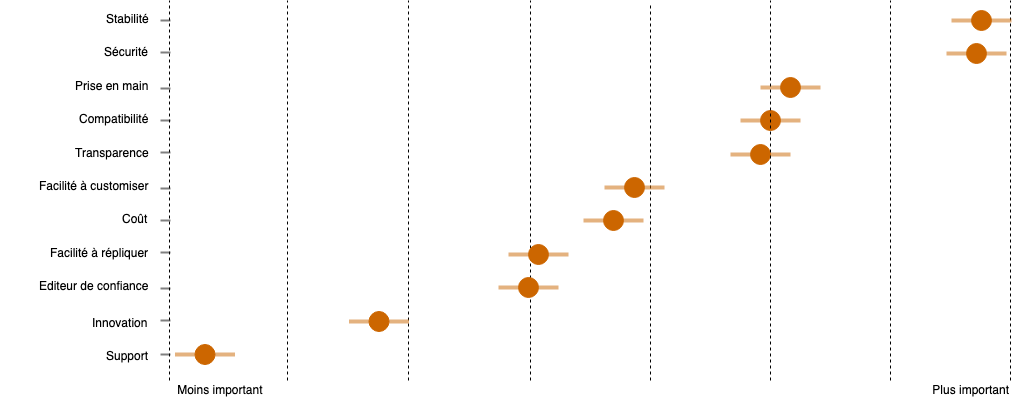
\includegraphics[scale=0.50]{./img/value_soft_os.png}
					\caption{Ce que les utilisateurs d'open source recherchent dans les logiciels}
   					\caption*{\color{silver}Source: opensourcesurvey.org}
				\end{figure}


	% --------------------------------------------------%
	%     												%
	%            Le marché de l'open source			    %
	%       										    %
	% --------------------------------------------------%

	\section{Le marché de l'open source} % in progress

		\paragraph{Libre n'est pas gratuit \\} 

			C'est bien l'un des principes de l'open source. Même si l'on y a pour vocation de s'étendre et de distribuer son produit, il est nécessaire, si ce n'est vital pour certains éditeurs de trouver une source de revenus pour leur logiciel.\\
			Il faut savoir qu'il existe une différence entre faire payer un logiciel propriétaire et un logiciel open source. 
			\begin{description}[font=\color{burntorange}]
				\item [Payer un logiciel propriétaire: ] permet non seulement d'apporter des revenus à une entreprise mais d'obtenir un « droit de possession », d'acquisition du logiciel.
				\item [Payer un logiciel open source: ] N'est pas un prix d'acquisition ni un droit d'utilisation mais une source de revenus à l'éditeur pour permettre au logiciel de prospérer.
			\end{description}

		\subsection{Les acteurs de l'open source}
			Il existe dans l'open source 4 grands acteurs:

			\begin{description}[font=\color{burntorange}]
				\item[Les fondations:] telles que Apache ou Eclipse, sont des organismes à but non lucratif qui stimulent et pilotent le développment de grands produits open source.
				\item[Les distributeurs:] Redhat, Canonical (Ubuntu) ou Mandriva sont des distributeurs (très souvent éditeurs par la même occasion). Ils sélectionnent des outils et composants autour d'un noyau Linux, en assurent le packaging, la distribution et le support
				\item[Les éditeurs:] Diffusent des logiciels sous licence open source, ils réalisent la promotion de leurs produits et proposent du support
				\item[Les prestataires: ] Ils vendent des services sur l'open source. Il peut s'agir de conseil, d'intégration, de support, de la formation, des solutions d'hébergement, etc.
			\end{description}

			Je m'intéresse particulièrement aux éditeurs de l'open source qui devront mettre en place des solutions pérénisant financièrement leur activité.\\

			Et de la prospérité les éditeurs en ont bien besoin car pour les autres acteurs, la taille, la mission et le produit présenté ne pose plus aucune difficulté de revenu. Doit-on encore se soucier du bon développement de Linux et de sa communauté ? Ces géants de l'open source, association à but non lucratif, ont des moyens marketings (plus de 60\% de leur revenus) et financier bien supérieurs aux éditeurs et prestataires qui restent pour la majorité des petites et moyennes entreprises.

			\emph{Comment fonctionne donc le modèle économique ou « business model » de ces entreprises ?}\\

		\subsection{Chez les éditeurs}

			Même s'ils bénéficient de l'open source pour réduire leur coût de ressources, celle-ci ne comblent pas les besoins de financement de la partie développement en interne, hébergement, marketing. Il est donc nécessaire de trouver des sources de revenus pour les éditeurs.

			Parmis celles-ci, on distingue 3 principales sources pour l'éditeur:

			\begin{itemize}[label=\textbullet, font=\LARGE \color{burntorange}]
				\item Vendre des licences
				\item Vendre du support
				\item Vendre de l'intégration
			\end{itemize}

			\subsubsection{Vendre des licences}

				Même s'il est interdit de faire payer l'utilisation d'un logiciel open source, les éditeurs ont bien compris commment faire bon usage de la « double licence ».

				\paragraph{Double licence commerciale\\}

					Il est possible de distribuer une œuvre dérivée utilisant le programme sans diffuser ses sources à l'aide d'une licence commerciale.\\
					Le programme officiel open source est gratuit mais sa version dérivée elle est payante à travers l'achat de licence commerciale.\\
					Pour l'entreprise MySql par exemple, la vente de licence représente plus de la moitié du \acrfull{ca}.

				\paragraph{Les extension payantes\\}

					L'éditeur peut proposer des extensions aux fonctionnalités présente dans le logiciel open source. Le logiciel initial est suffisemment de qualité et donne envie de payer quelques extension \textit{optionnelles} supplémentaire pour le confort et le besoin de l'utilisateur.

				\paragraph{Un support uniquement sur licence commerciale\\}

					Ici aussi, le logiciel est sous licence open source mais si l'on désire avoir le moindre support dessus, il faudra se tourner vers son confrère et sa licence commerciale.

			\subsubsection{Vendre du support}

				La prestation de support est une source principale de revenu pour l'éditeur, même s'il doit pour celà faire face à la concurrence potentielle de prestataires tiers que je précise juste après.

				Le support d'un logiciel inclut généralement :

				\begin{itemize}[label=\textbullet, font=\LARGE \color{burntorange}]
					\item L'accès privilégié aux correctif et ressources spécifique
					\item Une prise en chage des problèmes (anomalies, utilisation, mise en oeuvre ...)
					\item Des prestation d'audit, de certification, ou de prise de contrôle à distance, ainsi que la surveillance proactive et les corrections.
				\end{itemize}

				On peux distinguer différent modèles de financement concernant la vente de support:

				\paragraph{Uniquement le support\\}

					Certains éditeurs misent uniquement sur la vente de support. Le logiciel est gratuit mais le support lui est payant. Ce modèle de financement fonctionne pour certaines entreprises comme Tiny(OpenERP), Nuxeo.\\

					Le problème est qu'en cas ou le support n'a pas été utile l'année souscrite pour cause de stabilité du logiciel, le client voudra surement le résilier pour la suite.\\

					Plus le produit est de qualité, moins le support est facile à vendre car le client rencontre moins de difficultés.\\

					L'avantage est que plus on avance dans la technologie et plus la concurrence est présente on doit donc sortir des nouveautés constemment ce qui fragilise le produit et le rend instable.Le support est donc précieux dans le cadre professionnel.

				\paragraph{Faire payer la stabilité\\}

					Pour d'autre éditeurs, la stabilité d'un logiciel peut devenir source de profit. L'idée est de proposer deux logiciel:\\

					\begin{itemize}[label=\textbullet, font=\LARGE \color{burntorange}]
						\item Celui en licence open source sera classifié de « community edition ». Il sera présenté comme instable, pas entièrement testé, à ne pas déployer en production
						\item Tandis que le logiciel sous licence non-libre sera la licence sécurisée, une version « enterprise-ready », « fully tested ».
					\end{itemize} 

					Au final, la version community, c'est celle en cours de développement donc en avance de phase alors que la version entreprise c'est celle qui a été \textit{gelée} dans un état dit \textit{« stable »}.\\

					L'éditeur peut alors diffuser et promouvoir son produit à travers la version community, et apâter les entreprises dans la version payante ou généralement le support est packagé avec.\\

					L'éditeur jongle sur la stabilité de la version community en la rendant suffisamment stable pour donner envie de l'utiliser mais inciter fortement les entreprises à prendre la version sous licence commerciale qui sera accompagnée du support.

				\paragraph{Fonctionnalités avancées\\}

					Pour l'éditeur, un autre business model et celui de la fonctionnalitée avancée.\\
					La version community et enterprise n'est pas différente d'un point de vue stabilité mais ce sont les fonctionnalitées présente qui sont réduites sur la version community.\\

					Ceci permet de se dégager du paradigme « libre = instable » totalement infondé.\\

					La difficulté pour l'éditeur va être d'avoir suffisemment de fonctionnalitées pour rendre la version libre intéressante mais d'avoir une forte valeur ajoutée sur les fonctionnalités dans la version payante.

			\subsubsection{Vendre de l'intégration}

				Pour les éditeurs qui ne sont pas mondialement connu, il est possible de trouver la rentabilité en proposant l'intégration de son produit open source. C'est un moyen de démarrer dans le milieu sans trop de risque mais qui n'est pas « \gls{scalable} ». On ne peux s'étendre à l'étranger si l'on est le concurrent direct de ses intégrateurs partenaires. On reste donc sur un marché réduit.

			\subsubsection{Autres sources de revenus}

				\paragraph{Les campagnes de crowdfunding\\}

					En Mai 2019, la plateforme d'hébergement de logiciel Github, propose un programme de sponsoring et de crowdfunding.

				\paragraph{Vendre des extensions\\}

					Selon le modèle noyau-extension, nombre d'éditeur open source on trouvé leur part de marché dans la vente des extensions. Bien que réalisées généralement par la communauté, l'éditeur peut considérer la vente des extensions réalisées afin de rémunérer les contributeurs mais prélève un montant sur la vente d'extensions. De cette manière, l'éditeur de la solution open source Magento pour le e-commerce, prélève 30\% du prix de vente des extensions à la manière de l'Apple Store.

		\subsection{Communication par ses atouts}

			En guise de communication, l'open source n'a pas tant besoin de budget marketing. En effet il puise sa force là ou il a pris racine, c'est à dire dans sa communauté. Nul besoin de mettre de faux posts et avis sur touts les blogs du net, la vérité et la promotion de l'open source se fait principalement par la communauté.

			Le caractère open source permet en général de diffuser bien plus rapidement son produit.

			La communauté utilise donc tout support moderne de communication pour diffuser, twitter, poster ces informations

			Ainsi malgré le marketing ordinaire (campagne publicitaires, affiches, buzz-marketing ...) que ne peuvent se permettrent bon nombre d'éditeur, l'éditeur se doit d'\textbf{utiliser le marketing moderne 2.0}, qui est la force et le fondement de l'open source, pour prendre la relève.

	\paragraph{Les éléments clés à retenir}

		Afin de valoriser l'open source, nous pouvons utiliser différents leviers. 
		Autour de la communication, l'importance d'avoir un support clair de présentation, de documentation et de communication à l'aide d'outils efficaces.
		Dans l'organisation et la structuration du projet, il est important de veiller à ce que les parties prenantes constructrices du projet s'épanouissent dans leur domaine afin d'apporter la meilleure pierre à l'édifice. Côté management dans l'open source, l'intérêt est de se rapprocher de la communauté, lui faire confiance pour décider ensemble de l'avenir du projet par des méthodes de management horizontale en se mettant au même niveau que le groupe. Auprès du consommateur il faut noter l'importance d'écoute du besoin et de l'adaptation du projet à celui-ci, c'est le consommateur qui sollicite ensuite les principales sources de revenus comme le support logiciel.


\chapter*{\color{burntorange}{Etude terrain}} % 40 pages
	\section{Plateforme promotrice}
	\section{Gestion des ressources}
	\section{Chez le consommateur}
	\section{Marketing de l'open source}
\chapter{Confrontation} % 3 pages

% Confronter etat de l'art et etude terrain et donc Réponse aux hypothèse en disant validé à 80\% ...

\section{Promotion de l'open source}

	Ma première hypothèse concerne le manque de promotion, de mise en avant des produits open source, et du manque d'outil disponible sur les plateforme d'hébergement de code open source pour en faire le produit phare de tout les développeurs et entreprises du logiciel.

	\subsection{Des plateformes améliorables}

	Dans mon étude autour de l'open source, je me suis aperçu de la multitude des plateformes disponibles pour présenter les projets open sources et permettre la contribution. Malgré celà, il me semblait nécessaire de mettre en place une interface pour accueillir les potentiels futur contributeur, une vitrine permettant de visualiser le produit.

	Avec l'étude terrain et les résultat à mes questions autour de ce sujet, je me suis aperçu que les plateformes n'ont pas nécessité à promouvoir le projet car l'aspiration à la contribution n'est pas lié à la motivation et au marketing qui gravite autour. C'est sur besoin qu'a le consommateur à utiliser une spécificité du logiciel open source, et donc à communiquer son idée, ses besoins pour  et orienter le développement du produit vers son besoin.

	Ainsi mon hypothèse sur l'interface de promotion des projets open source n'est pas valide.

	Néanmoins il s'en est dégagé un besoin crucial d'améliorer la communication entre toutes les parties prenantes du projet open source.

	\subsection{Le marketing de l'open source}



\paragraph{Réponse à l'hypothèse}

\section{Optimisation des ressources}

	\subsection{Business model de l'open source}

	\subsection{Gestion des ressource humaines}

\paragraph{Réponse à l'hypothèse}

\section{Envies et besoins de contribuer}

	Ma troisième hypothèse traite du manque de sensibilisation qui plane sur l'open source, faisant de celui-ci un sujet de malentendu, d'incompréhension ou d'ignorance par les consommateurs potentiel. Si l'on sensibilisait plus le consommateur de l'open source sur l'importance de leur contribution, alors le blason de l'open source en serait redoré et attirerait encore plus de monde.

\subsection{Sensibiliser le grand public}

	Lors de mes recherches autour de l'open source et en comparant avec mon vécu dans mes entreprises et à l'école, je me suis aperçu du manque de sensibilisation sur le vaste sujet qu'est l'open source.\\

	Il est vrai que je n'ai que vaguement entendu ce sujet à quelques reprises avant d'en faire mon sujet d'étude.
	J'ai donc profité de mon étude terrain pour aller questionner d'autres personnes sur ce sentiment de manque d'information autour de l'open source.\\
	Je confirme donc mon hypothèse sur le fait que l'on entend pas parler de l'open source pour le grand public car c'est le meme ressenti qui est partagé par les personnes interviewé et ayant répondu au questionnaire.\\

	Pour autant lors de mes différents échanges, je m'aperçoit que la cible du grand public est erronée. En effet, l'open source est généralement à destination des développeurs, des entreprises et dans ce monde là, on est normalement sensibilisé à l'open source.\\

	C'est une erreure d'interprétation que j'ai eu en faisant l'amalgame du consommateur et de l'utilisateur final du produit. Les utilisateurs finaux (ou grand public) ne sont pas forcément développeurs, et les produits open source ne sont pas tous des logiciels à destination de ces utilisateurs.\\

	L'open source s'adresse donc principalement à son consommateur qui est généralement développeur et qui, pour des besoins d'entreprise ou personnel, va utiliser ces briques logicielles afin d'éviter de réinventer la roue.\\

	Ainsi s'il n'est pas nécessaire de sensibiliser le grand public, il n'en est pas de même pour les entreprises.

	\subsection{Sensibiliser l'entreprise et le contributeur}

	En entreprise, le sujet de l'open source est considéré comme très important, on en entend parler, on l'utilise même beaucoup et c'est ce que j'ai pu constater également de mon coté mais aussi par les échanges que j'ai eu auprès des interviews.\\

	Les personnes concernés ont acquiescé le fait que l'entreprise à besoin de l'open source, qu'elle s'attend à ce que les développeur s'y connaissent sur le sujet... Pour autant, ils ne souhaitent pas forcément apporter leur pierre à l'édifice.\\

	Aujourd'hui, il est donc important de sensibiliser les entreprises et de trouver le moyen de les faire contribuer au monde du logiciel ouvert.

	En effet, la contribution de l'entreprise est un axe exponentiel de croissance pour l'open source.\\

	Une entreprise qui contribue en ouvrant son code, sera sensible au autres entreprises qui en ont fait de même. Il sera alors plus facile pour elles de permettre à leurs développeur de contribuer à l'open source tant pour améliorer leur propres code en interne que pour utiliser celui des autres et l'adapter à ses besoins.\\

	Le développeur contributeur sera donc sensibilisé à son tour.

\paragraph{Réponse à l'hypothèse}



\chapter{\color{burntorange}{Transposition}}

\chapter*{\color{burntorange}{Conclusion}}

\end{document}